\chapter{Results and Analysis}
The numerical results are displayed in this chapter for both parachute simulation and DNS of cloud entrainment process. In each part, the experimental setups are firstly introduced, and then the numerical results and quantitative analysis are presented.

\section{Results for parachute simulation}
This section aims to demonstrate the improvements and features of the new parachute model. Firstly, the experimental setup are introduced including the domain size, boundary conditions, and the initialization of parachute canopy and flow field. Then the turbulent-viscosity models are incorporated to the current code and compared with the laminar-version simulation. In the meanwhile, we try to investigate the new porosity model, and compare its effects with the previous non-porous parachute. Finally, the collision handling modules are applied to simulate the fabric collision and folding procedure.
 
\subsection{Experimental setup}
The experiments are carried out in a wind tunnel, which is set to be $14m\times14m\times 40m$ as default with constant velocity at the inlet, outflow boundary condition with pressure $p = 0$ $Pa$ at the outlet, and periodic boundary condition for the rest of faces. In some situations, the periodic boundary condition can be replaced by the non-slip boundary condition or wall boundary condition. The domain size may also change for some specific reasons. As for the parachute types, we consider several descending round canopies: C-$9$, G-$11$, G-$12$, G-$14$ and T-$10$. 

The C-$9$ type parachutes are used in the Advanced Concept Ejection Seat (ACES) in all current U.S. jet fighters and personal parachutes in cargo airplanes. It has $8.5m$ nominal diameter, $28$ number of gores, $7m$ suspension lines. 
The G-$11$ $100$-feet parachute is heavy capacity cargo parachute designed primarily for used in the aerial delivery of vehicular and bulk-type platform loads. It has $30.3m$ diameter, $120$ suspension lines with length of $10.6m$. Each $10$ of the consecutive suspension lines are connected to a suspension riser, and thus giving $12$ suspension risers with length of $18.28m$. These suspension risers are further evenly divided into three suspension riser assemblies terminating in three riser attaching loops. 
The G-$12$ $64$-feet cargo parachute is designed for medium capacity use with the A-$22$ air delivery cargo bag. It has the similar structure as G-$11$ while with $64$ suspension lines of $15.5m$ and $8$ risers of $18.2m$. 
The G-$14$ $34$-feet cargo parachute provides the capability to deliver non-fragile supplies and equipment using low-velocity air delivery method. It can also be assembled to a cluster of three to support payloads up to $1500$ $lbs$. It has $32$ suspension lines of length $8.3m$ with two risers. 
The T-$10$ $35$-feet personnel parachute is designed for combat mass-assault airborne operations and training. It is a parabolic-shape and has a nominal diameter of $10.7m$ with $30$ suspension lines. The technical specifications for these canopies are listed in \Table{parachute_specification}, and \Figure{init_parachutes} illustrates the scales and initial shapes of different types of parachutes. The strings attached to the canopies of G-$11$ and G-$12$ reflect the result of combined effects of suspension lines and riser lines.
\begin{table}
\centering
\begin{tabular}{lcccc}
\hline\hline
Type   & Diameter & Shape 		  & Suspensions        & Risers \\
\hline
C-$9$  & $8.5m$   & flat circular & $28\times 7m$     & none   \\
G-$11$ & $30.3m$  & flat circular & $120\times 10.6m$ & $12\times 18.2m$ \\
G-$12$ & $19.5m$  & flat circular & $64\times 15.5m$  & $8\times 18.2m$ \\
G-$14$ & $10.3m$  & flat circular & $32\times 8.3m$   & $2\times 0.76m$ \\
T-$10$ & $10.7m$  & parabolic     & $30\times 8.5m$   & $2\times 0.76m$\\
\hline
\end{tabular}
\caption{The technical specifications of parachutes}\label{parachute_specification}
\end{table}

\begin{figure}[!htbp]
\centering
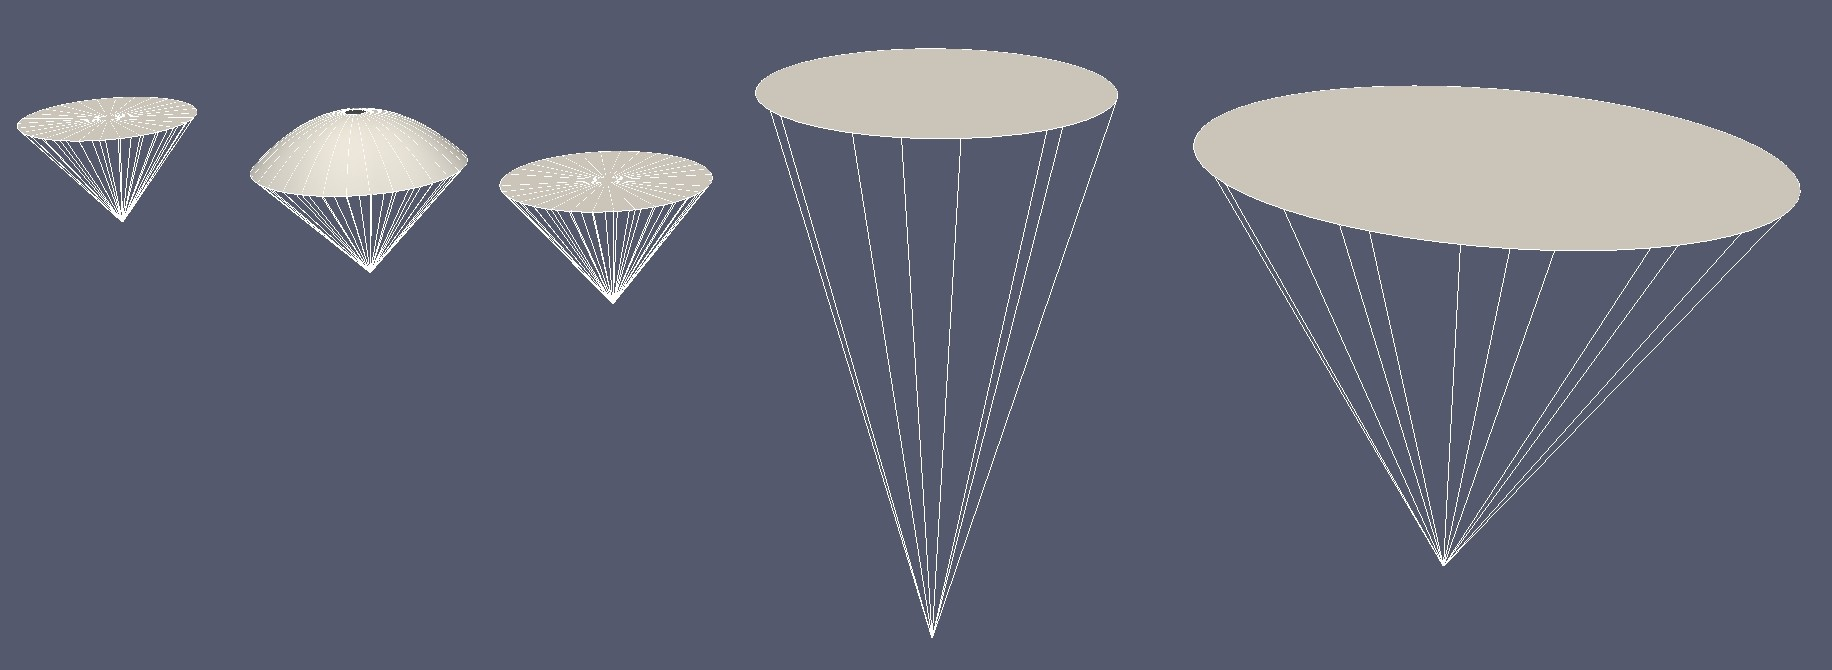
\includegraphics[width=\textwidth]{Figures/init_parachutes.jpg}
\caption{Initial shapes of parachutes, from left to right are C-$9$, T-$10$, G-$14$, G-$12$, G-$11$.}\label{init_parachutes}
\end{figure}

The computational mesh consist of two parts: the Eulerian mesh of fluid field and Lagrangian mesh of the parachute canopy. The fluid field is computed in a three-dimensional rectangular grid with uniform grid spacing. Various resolutions are tested depending on the domain size and the required accuracy. The canopies' mesh is generated by CGAL $2$D triangulations package \cite{CGAL_Triangulation} based on the constrained Delaunay triangulation. The computational mesh of T-$10$ parachute is displayed in \Fig{T10-mesh} for illustration.
\begin{figure}[!htbp]
\centering
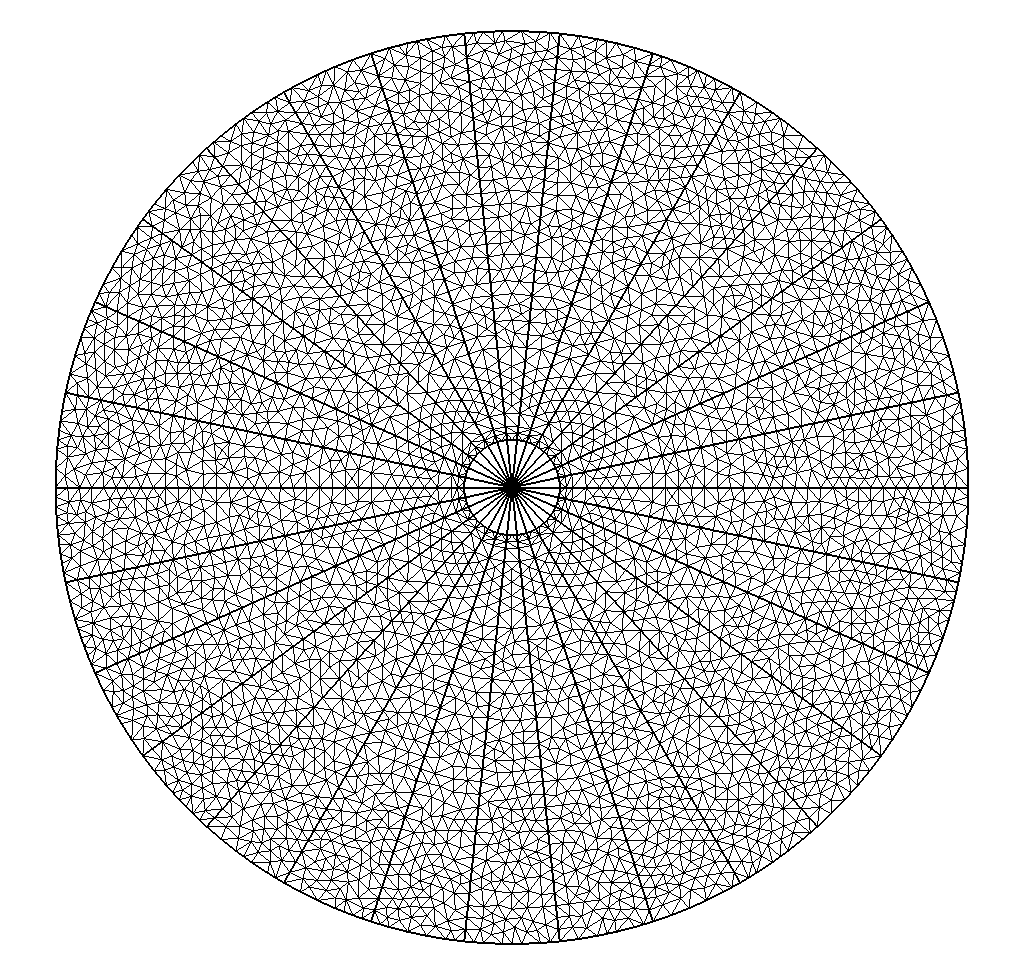
\includegraphics[width=0.3\textwidth]{Figures/T10-mesh-top.png}
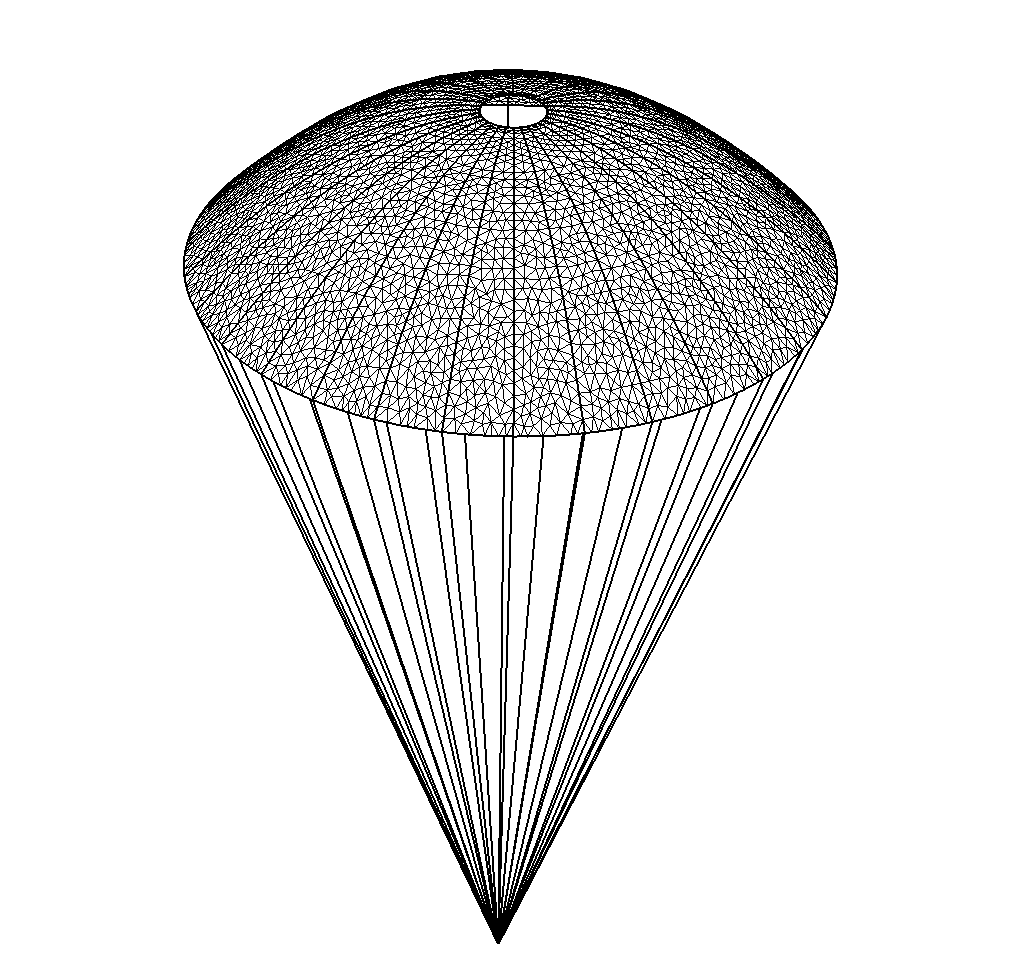
\includegraphics[width=0.3\textwidth]{Figures/T10-mesh-front.png}
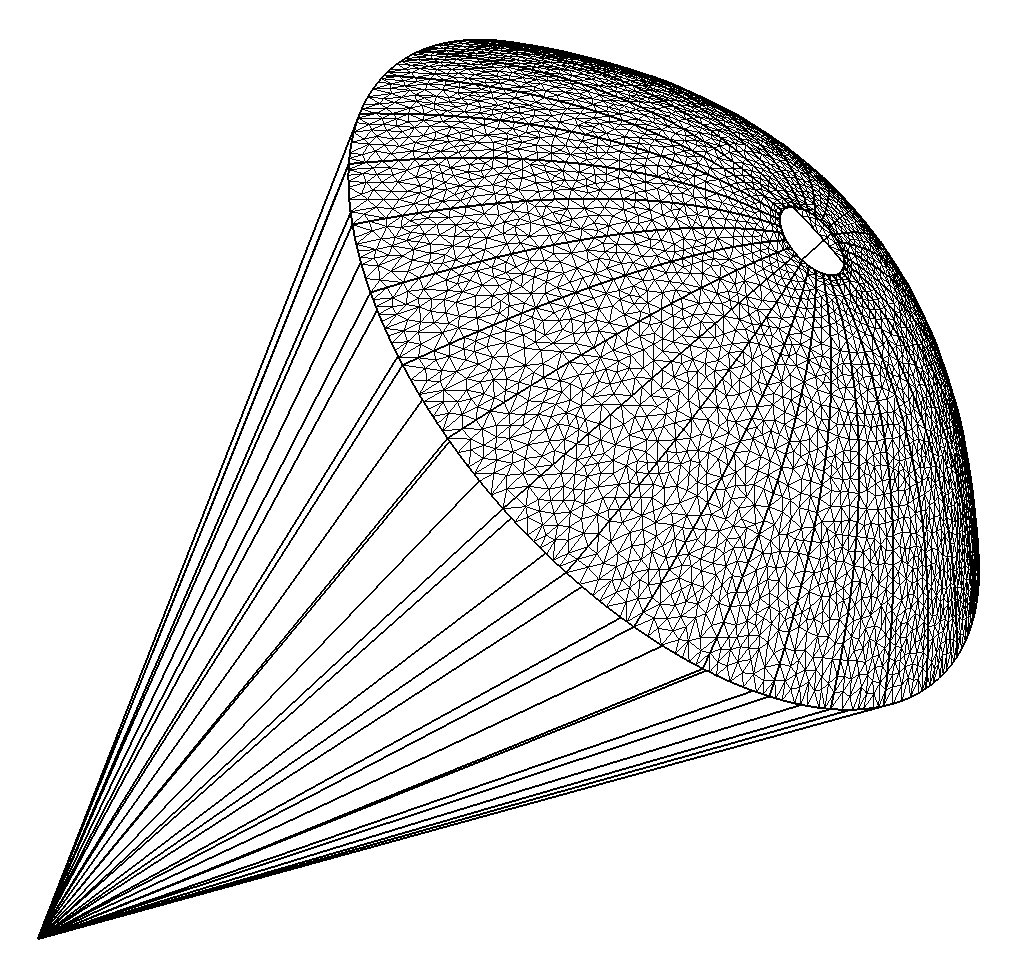
\includegraphics[width=0.3\textwidth]{Figures/T10-mesh-rear.png}
\caption{Initial mesh of T-$10$ canopy.}\label{T10-mesh}
\end{figure}

Two major settings have been applied in the wind tunnel: the drop test and the fixed-end test. In the drop test, the parachute is released at the top of the wind tunnel from either folded or unfolded shapes, and then the parachute freely falls in the tunnel until it hits the ground. This experiment aims to simulate the inflation stage of the parachute falling and study the factors affecting this procedure. The settings of drop test is close to a real situation, it, however, may terminate before the parachute reaching the stable state. Instead of free falling, the fixed-end test fixes one end of the parachute, and let the wind blow into the tunnel to inflate the canopy. This test can be used to measure the drag force on the canopy and is able to run arbitrarily long until the drag becomes stable.
  
\subsection{Turbulent-viscosity models}
The Reynolds number around a full-size parachute usually exceeds several millions, and hence the fluid flow has to be treated as turbulence \cite{Johari05}. The turbulent-viscosity models is one of many approaches to simulate the turbulent effects. In the current parachute simulation, a two-equation model has been developed attempting to duplicate several features during the turbulence-parachute interactions. The principle of the two-equation model is to modify the viscosity coefficient in the Reynolds-averaged Navier-Stokes equation, so as to approximate the effects of Reynolds stresses. The turbulent viscosity is computed from turbulence quantities such as $k$ and $\varepsilon$, which are solved from a couple of transport equations. In this section, three types of $k-\varepsilon$ model, standard, Re-Normalisation Group (RNG), and realizable turbulence model are investigated in the parachute drop test, and meanwhile compared with the simulation results without using turbulence model, in which the viscosity is a constant. The velocity magnitude and turbulence viscosity for each model are recorded. 

\Fig{turbulent_visc_vel_3ms} shows the velocity magnitude and turbulent viscosity for different models at the same time frame. When the inlet velocity is $3m/s$, it shows that all the $k-\varepsilon$ models produce similar flow patterns, and they also resemble the pattern in the simulation without using turbulence model. However, the standard model tends to predict higher velocity magnitude than the RNG model and Realizable model and the flow patterns near the parachute vent are significantly different. As for the turbulent viscosity, the standard model resembles the pattern of RNG model while its numeric value is one order of magnitude larger. It is interesting to see that, in the realizable model, the viscosity after the parachute canopy is significantly smaller than the other two models. This is because the realizable model predicts higher turbulence dissipation rate $\varepsilon$ in the parachute wake, and thus the viscosity quickly decreases according to the formula $\mu_{t} = C_{\mu}\rho k^2/\varepsilon$.

\Fig{turbulent_visc_vel_10ms} shows the same test, yet with inlet velocity $10m/s$. It is reasonable that the parachutes are subjected to stronger drag force than the case of $3m/s$, and hence falls much slower. The Realizable model still predicts the smallest value of the viscosity in the wake of the parachute. However, since the inflow velocity increases, the kinetic energy and dissipation rate produced at the inlet are able to propagate further and dominate the viscosity field. As the parachute falls and interacts with the inlet flow, it pushes the turbulent viscosity field away to each side and generates vortex-like pattern \cite{Johari05}.

\Fig{turbulent_visc_vel_15ms} displays the velocity and viscosity field with inlet velocity $15m/s$. This test gives a real turbulence field, and therefore the predictions of the three models are expected to be reasonable. The viscosity field predicted by the RNG model resembles the standard one but with more details in the wake, while the realizable model produces a completely different viscosity field. This field results in a more chaotic velocity field than the other two cases. We also notice that using turbulence model makes the parachute drop significantly faster than the case without turbulence model. This can be explained by the fact that the turbulence viscosity plays as a friction between fluid elements, and hence reduce the velocity magnitude and the drag force.

In summary, the standard $k-\varepsilon$ model assumes that the flow is fully turbulent, and the effects of molecular viscosity are negligible. This model was demonstrated to work fairly well for a wide range of wall-bounded and free shear flows. However, since the parachute canopy prevents the flow from passing through and the flow behind the parachute is less-turbulent when the inlet velocity is small, the standard model tends to overestimate the turbulent viscosity in the parachute wake. The RNG model is integrated to obtain an accurate description of how the effective turbulent transport varies with the effective Reynolds number, allowing the model to better handle low-Reynolds-number and near-wall flows. The RNG model is expected to be more responsive to the effects of rapid strain and streamline curvature than the standard model. Hence in the rapidly strained flows, it yields a lower turbulent viscosity than the standard model. The Realizable model is proposed by satisfying certain mathematical constrains on the normal stresses, consistent with the physics of turbulent flows. It is believed that the modified form of the equation for $\varepsilon$ better represents the spectral energy transfer. The performance of the model has been found to be substantially better than that of the standard model.

\begin{figure}[!htbp]
\centering
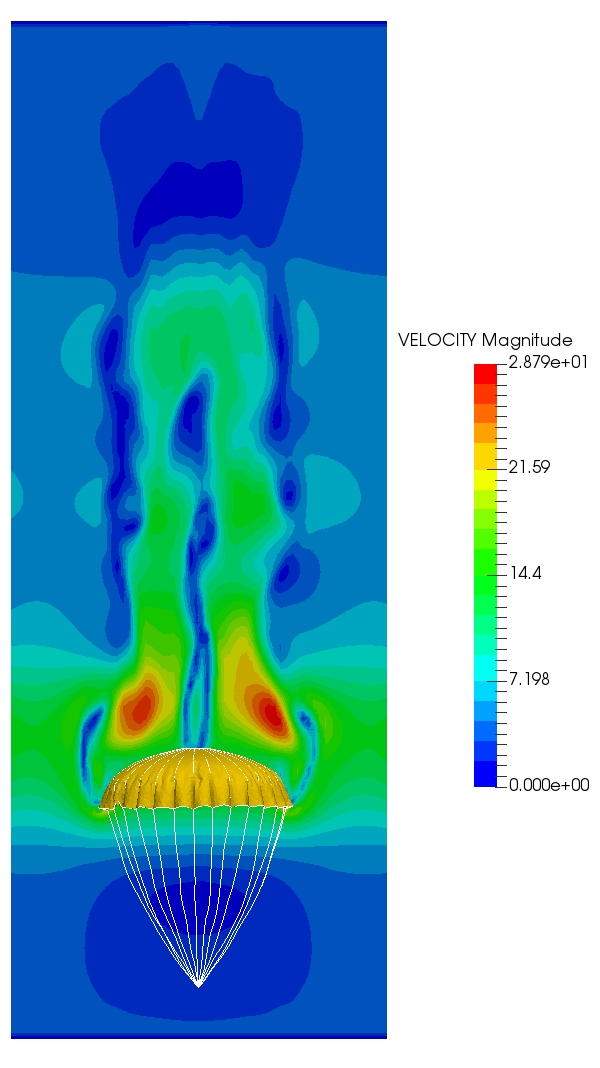
\includegraphics[width=0.24\textwidth]{Figures/c9-vel-std-3ms.jpg}
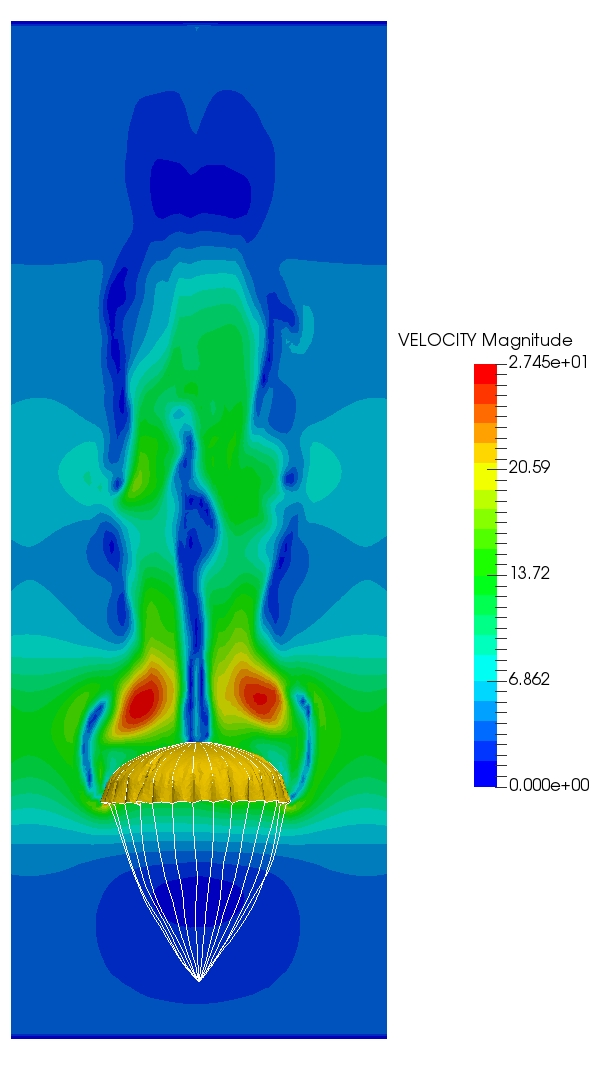
\includegraphics[width=0.24\textwidth]{Figures/c9-vel-rng-3ms.jpg}
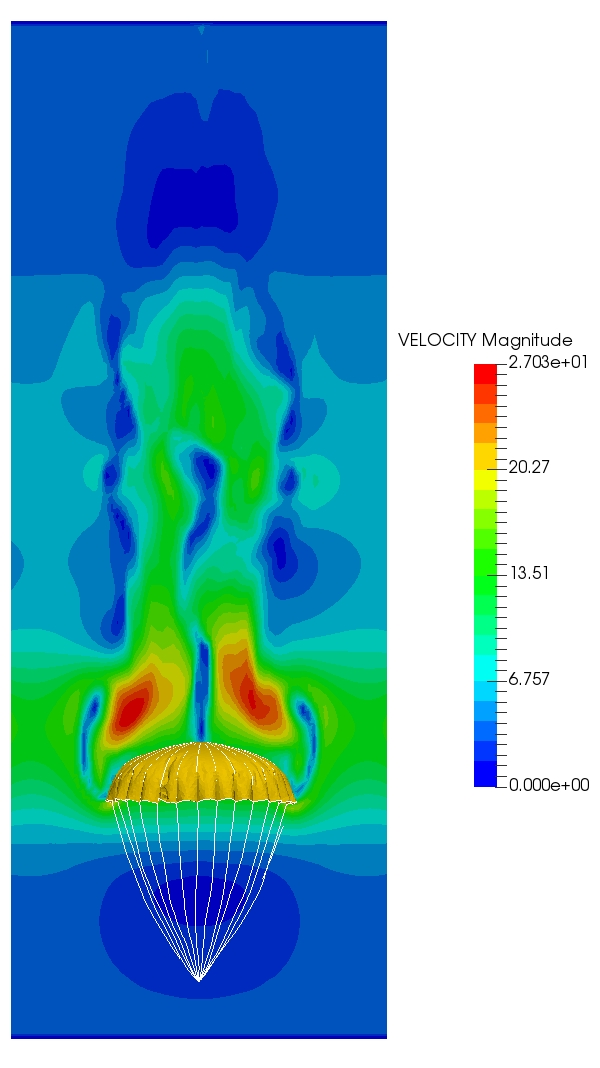
\includegraphics[width=0.24\textwidth]{Figures/c9-vel-real-3ms.jpg}
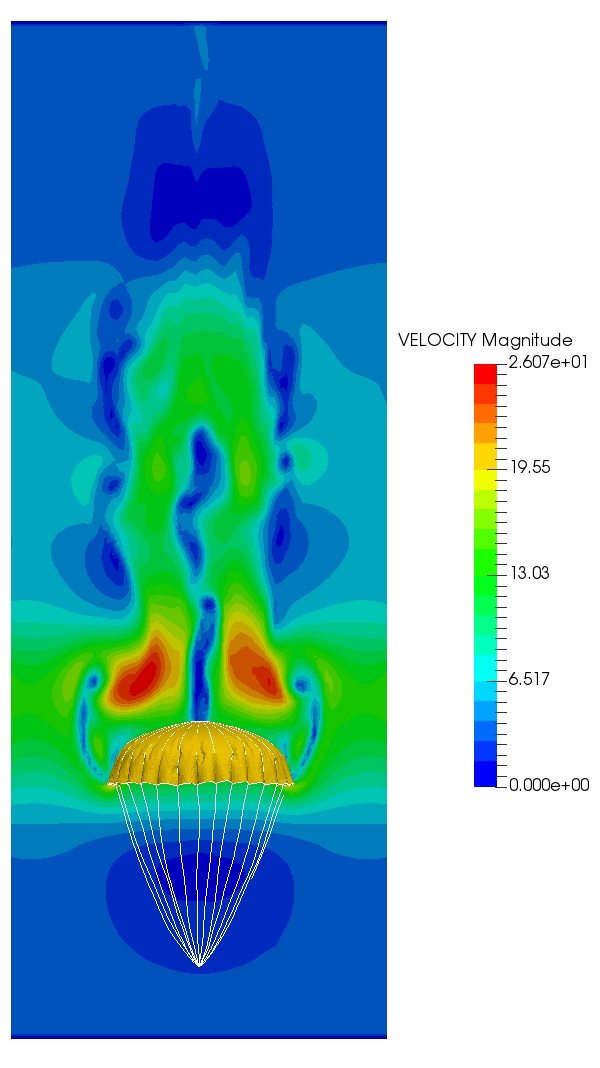
\includegraphics[width=0.24\textwidth]{Figures/c9-vel-lam-3ms.jpg}\\
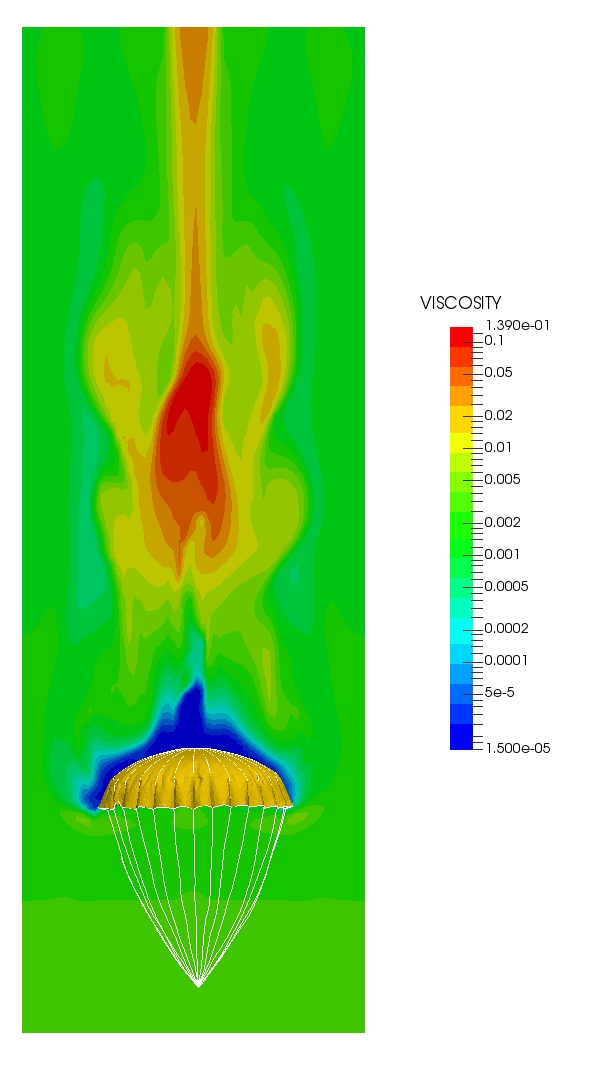
\includegraphics[width=0.24\textwidth]{Figures/c9-vis-std-3ms.jpg}
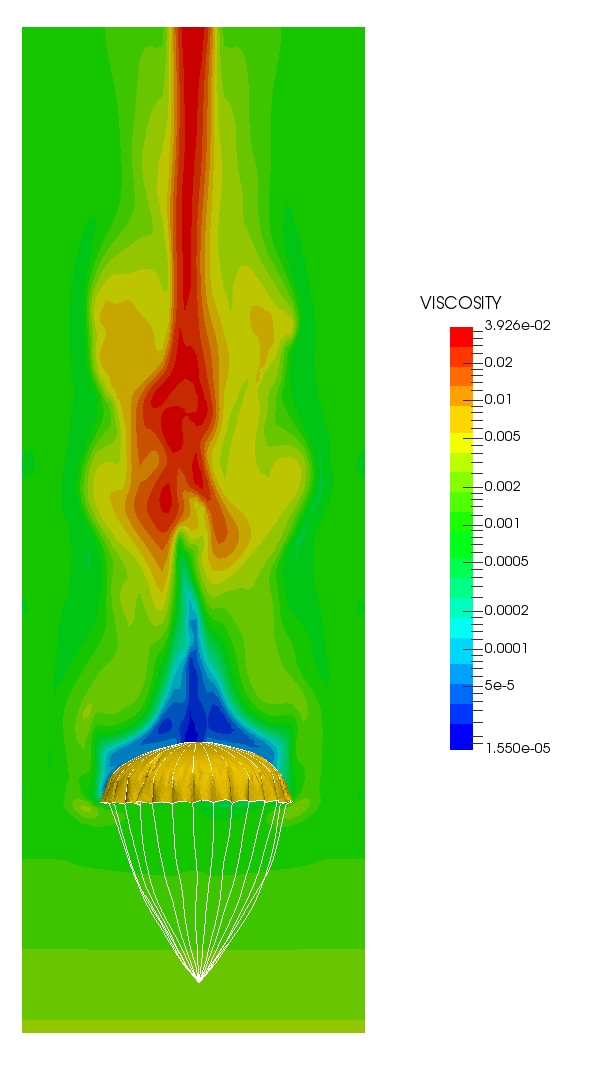
\includegraphics[width=0.24\textwidth]{Figures/c9-vis-rng-3ms.jpg}
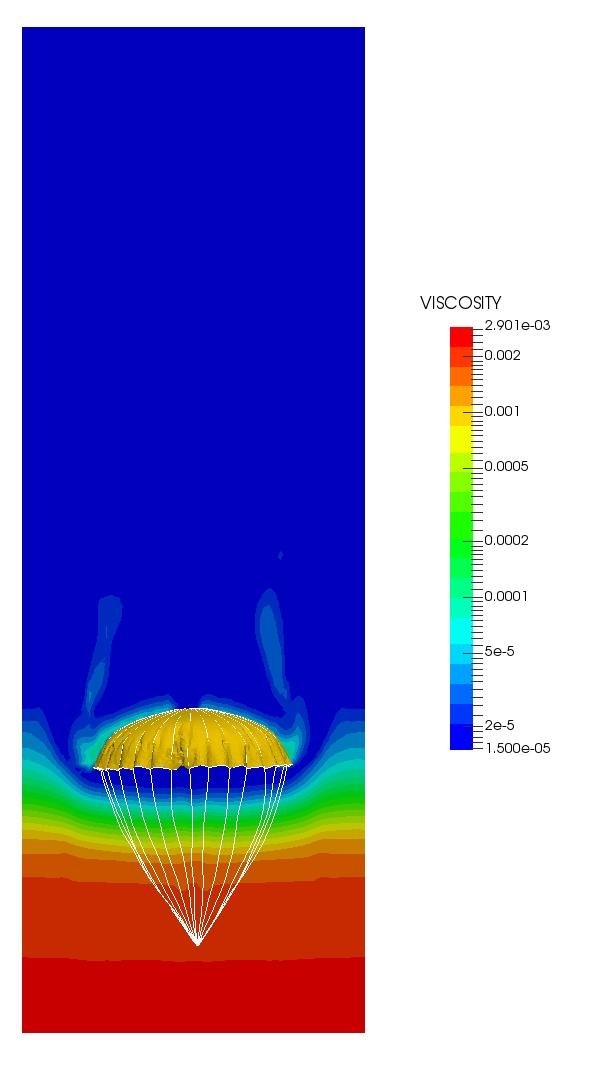
\includegraphics[width=0.24\textwidth]{Figures/c9-vis-real-3ms.jpg}
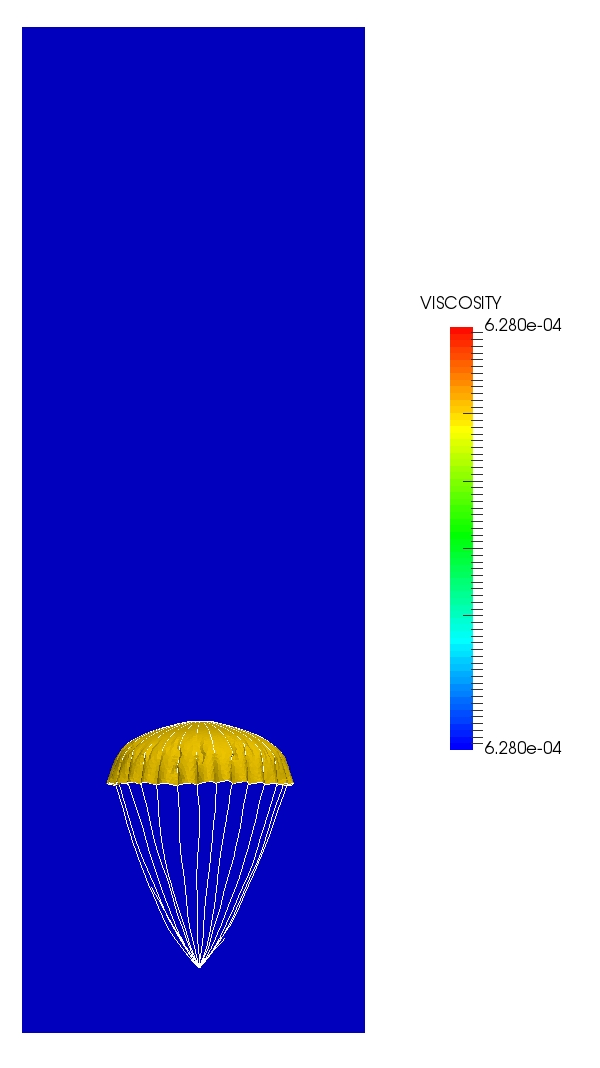
\includegraphics[width=0.24\textwidth]{Figures/c9-vis-lam-3ms.jpg}
\caption{Velocity magnitude and turbulent viscosity for C-$9$ parachute using different turbulent models at the same time frame. The inlet velocity is $3m/s$. The figures in the upper row displays the velocity magnitude and the figures in the lower row shows the turbulent viscosity.}
\label{turbulent_visc_vel_3ms}
\end{figure}

\begin{figure}[!htbp]
\centering
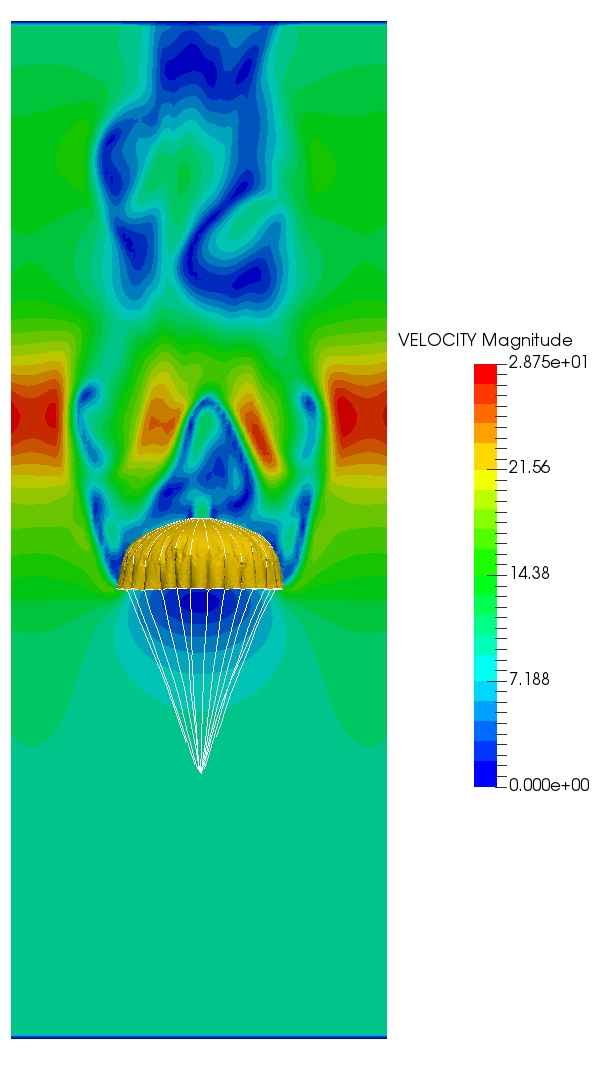
\includegraphics[width=0.24\textwidth]{Figures/c9-vel-std-10ms.jpg}
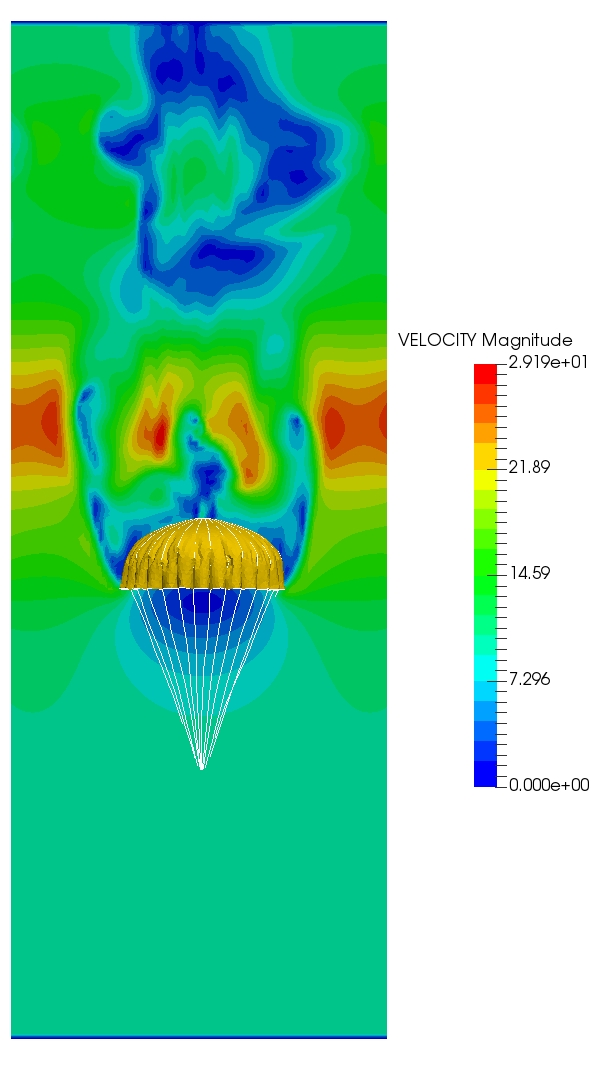
\includegraphics[width=0.24\textwidth]{Figures/c9-vel-rng-10ms.jpg}
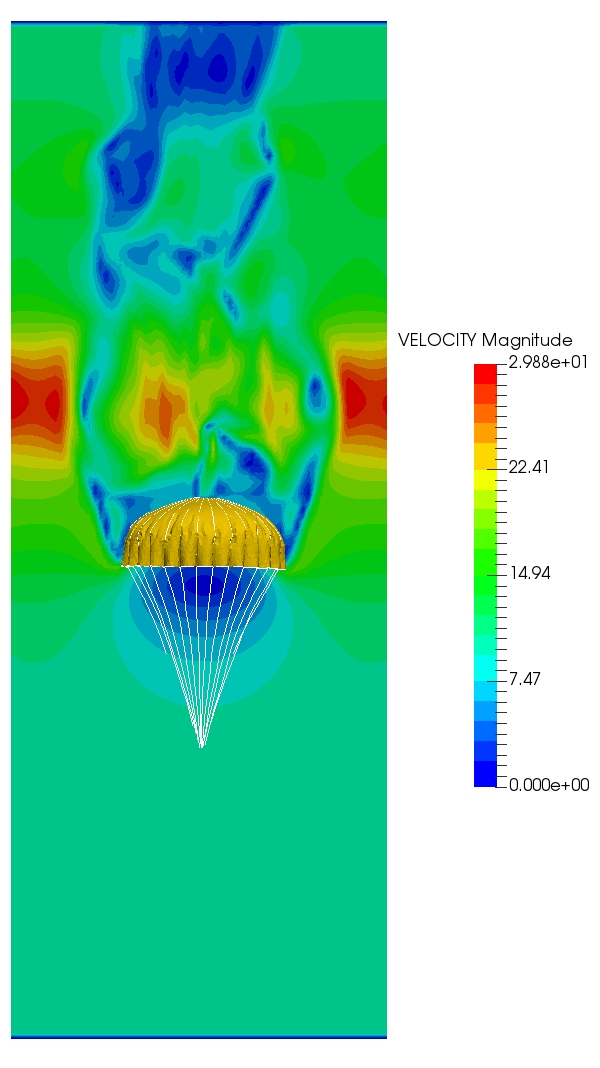
\includegraphics[width=0.24\textwidth]{Figures/c9-vel-real-10ms.jpg}
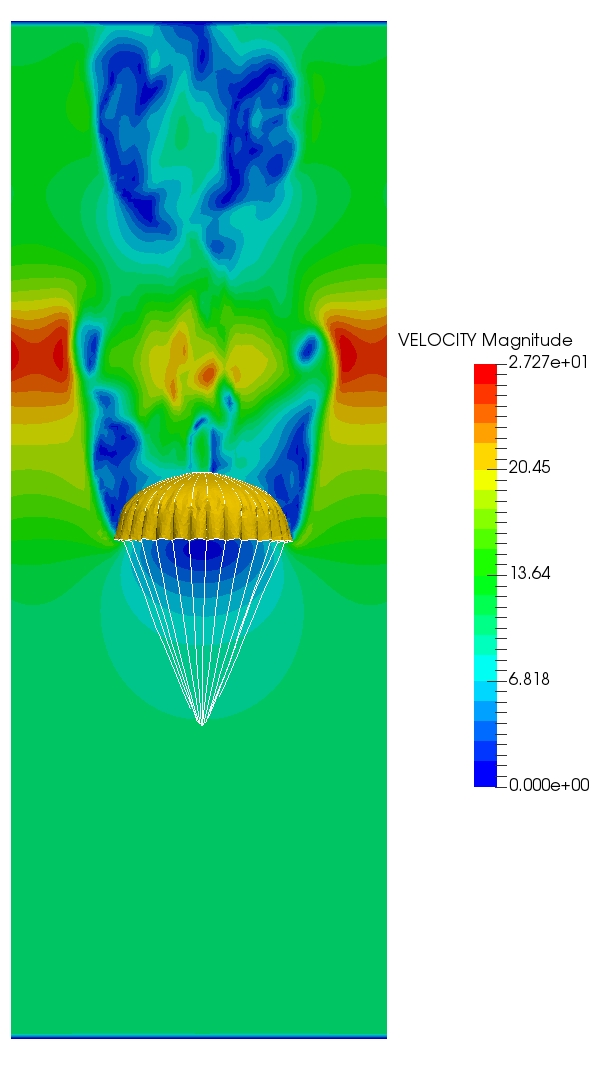
\includegraphics[width=0.24\textwidth]{Figures/c9-vel-lam-10ms.jpg}\\
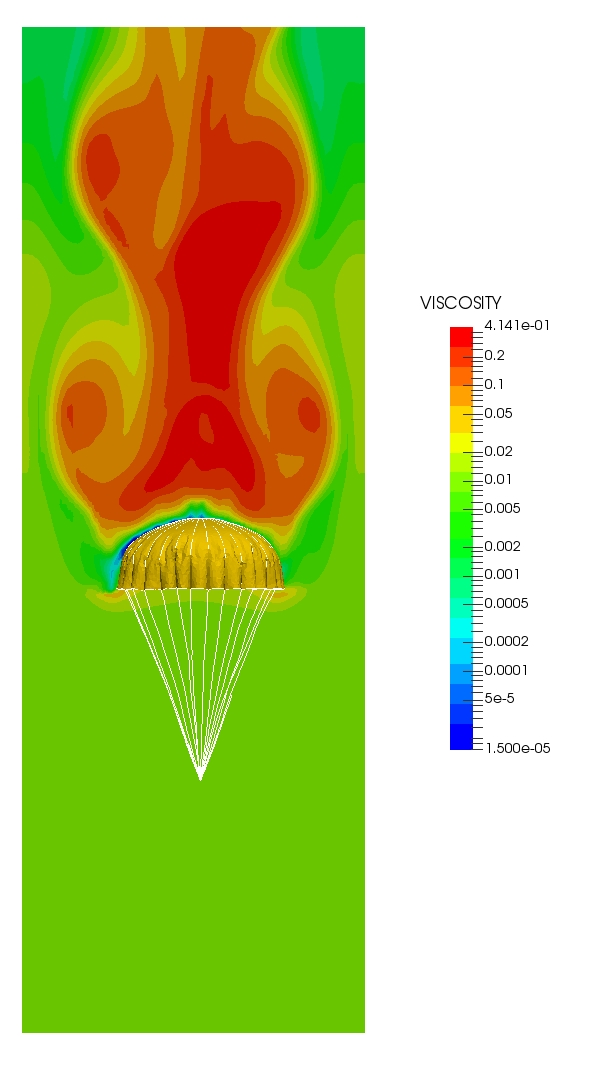
\includegraphics[width=0.24\textwidth]{Figures/c9-vis-std-10ms.jpg}
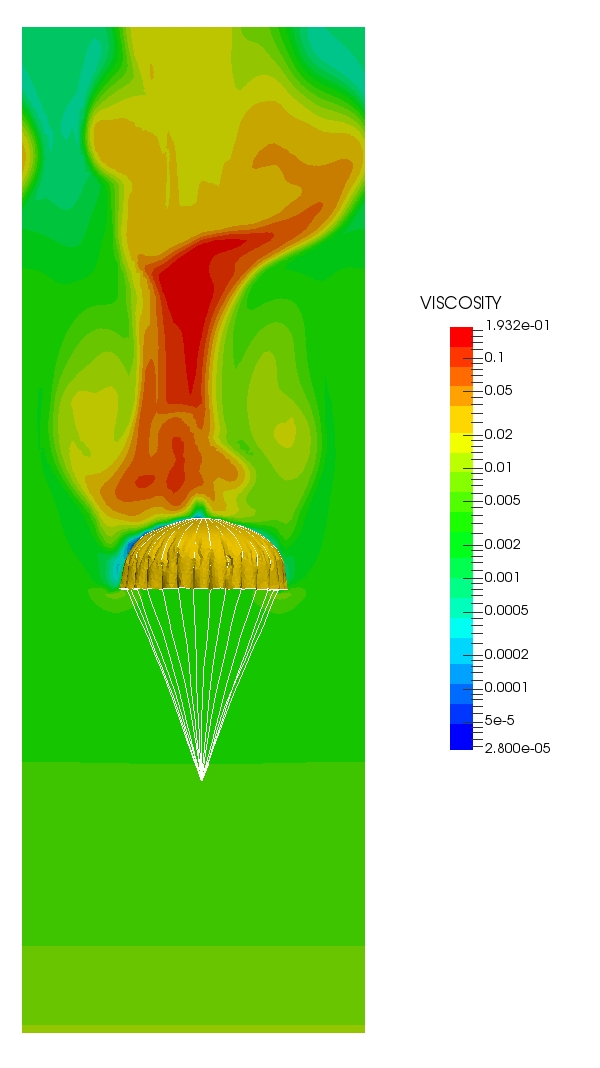
\includegraphics[width=0.24\textwidth]{Figures/c9-vis-rng-10ms.jpg}
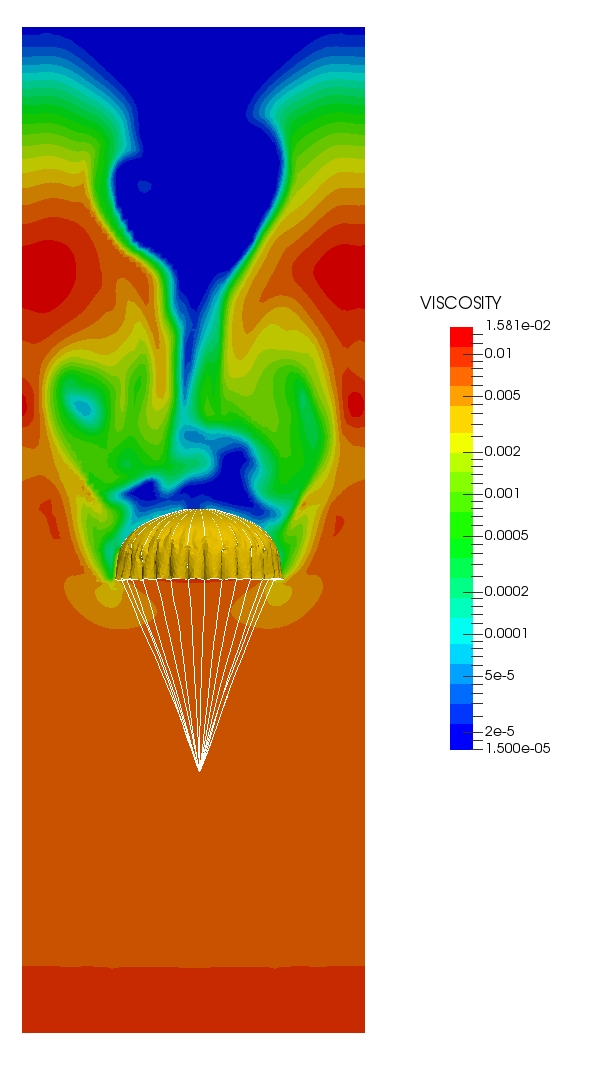
\includegraphics[width=0.24\textwidth]{Figures/c9-vis-real-10ms.jpg}
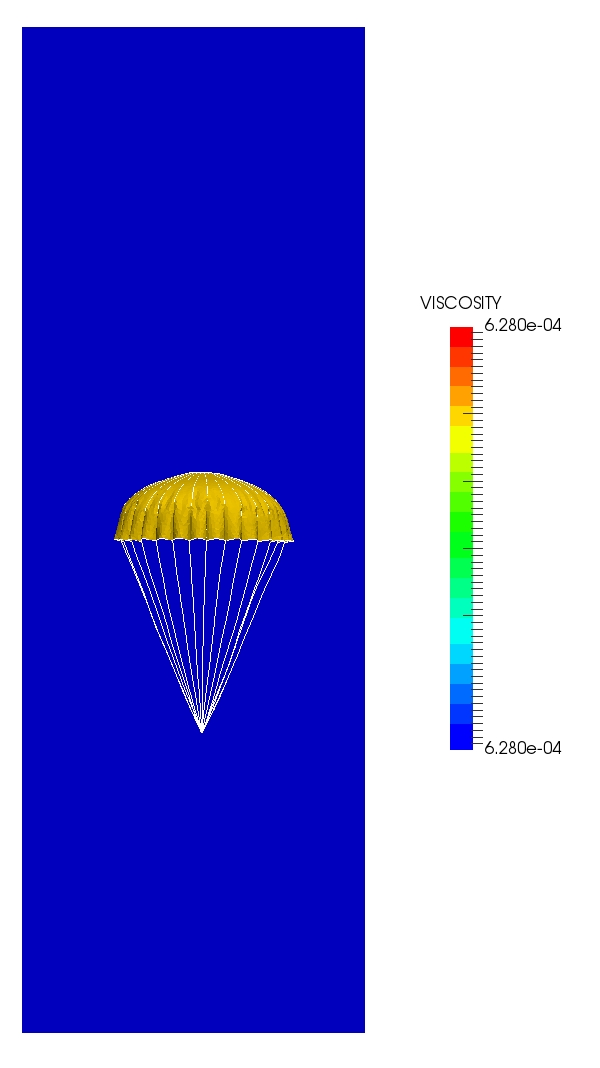
\includegraphics[width=0.24\textwidth]{Figures/c9-vis-lam-10ms.jpg}
\caption{Velocity magnitude and turbulent viscosity for C-$9$ parachute using different turbulent models at the same time frame. The inlet velocity is $10m/s$. The figures in the upper row displays the velocity magnitude and the figures in the lower row shows the turbulent viscosity.}
\label{turbulent_visc_vel_10ms}
\end{figure}

\begin{figure}[!htbp]
\centering
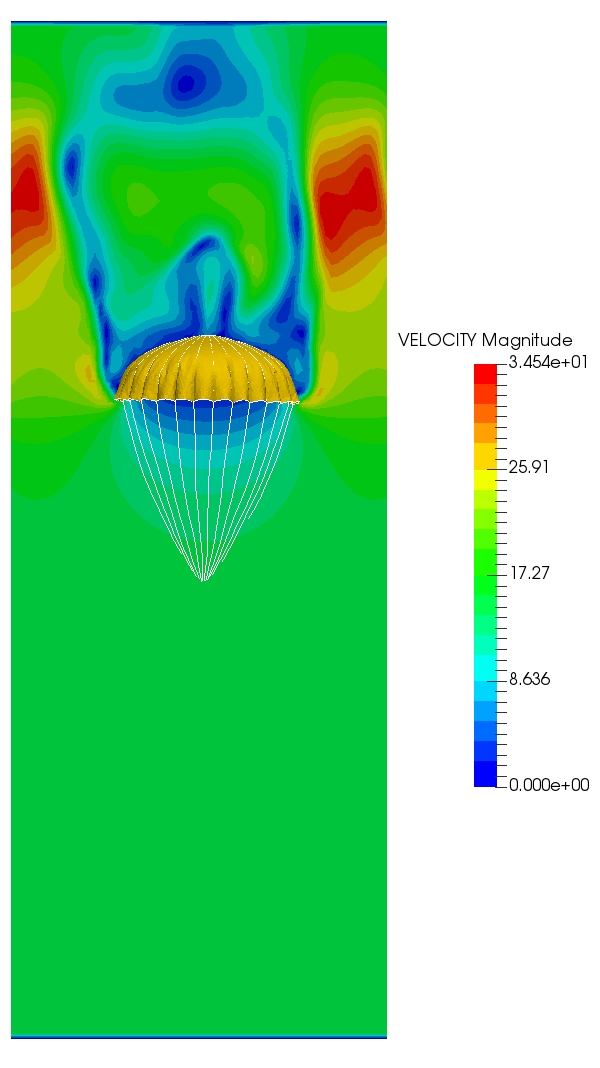
\includegraphics[width=0.24\textwidth]{Figures/c9-vel-std-15ms.jpg}
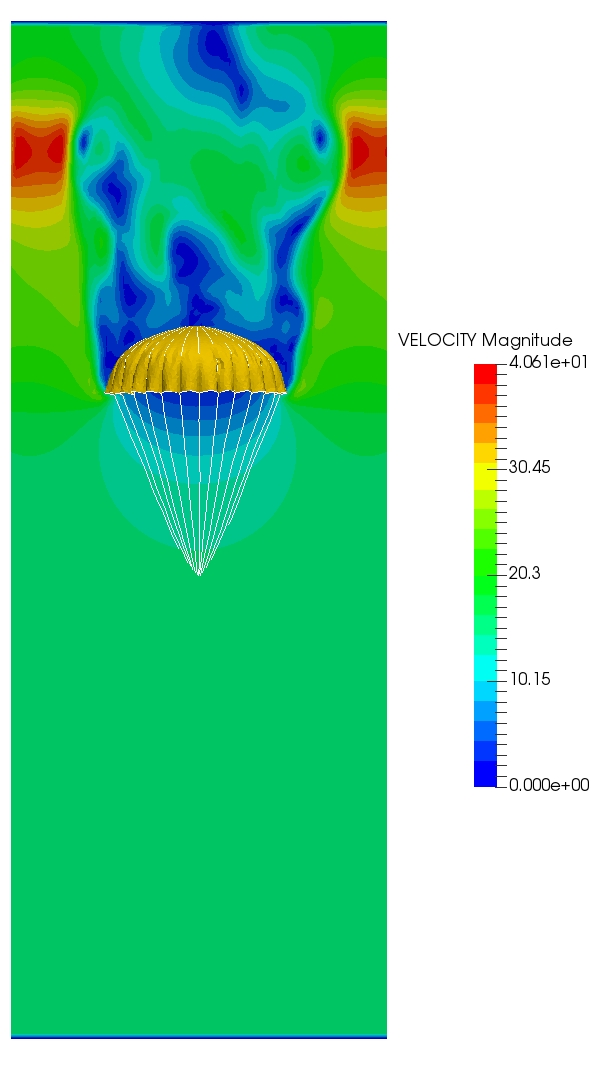
\includegraphics[width=0.24\textwidth]{Figures/c9-vel-rng-15ms.jpg}
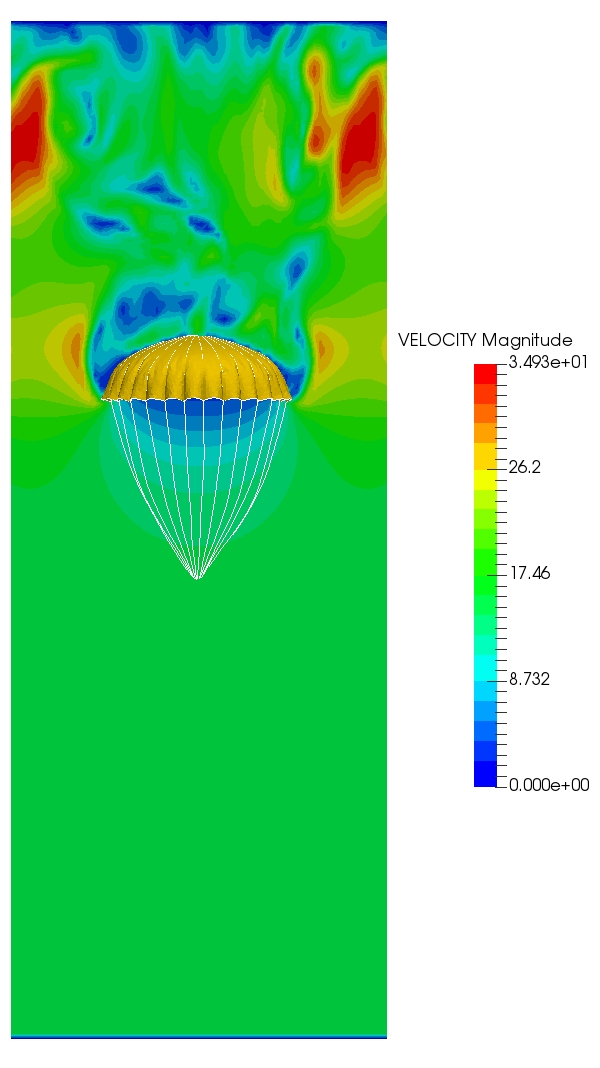
\includegraphics[width=0.24\textwidth]{Figures/c9-vel-real-15ms.jpg}
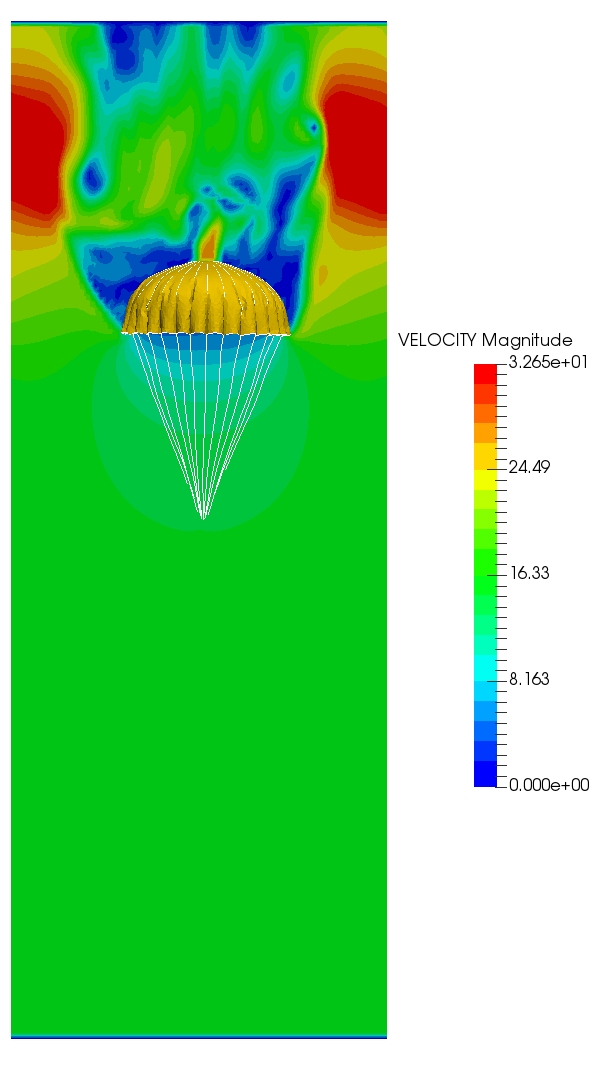
\includegraphics[width=0.24\textwidth]{Figures/c9-vel-lam-15ms.jpg}\\
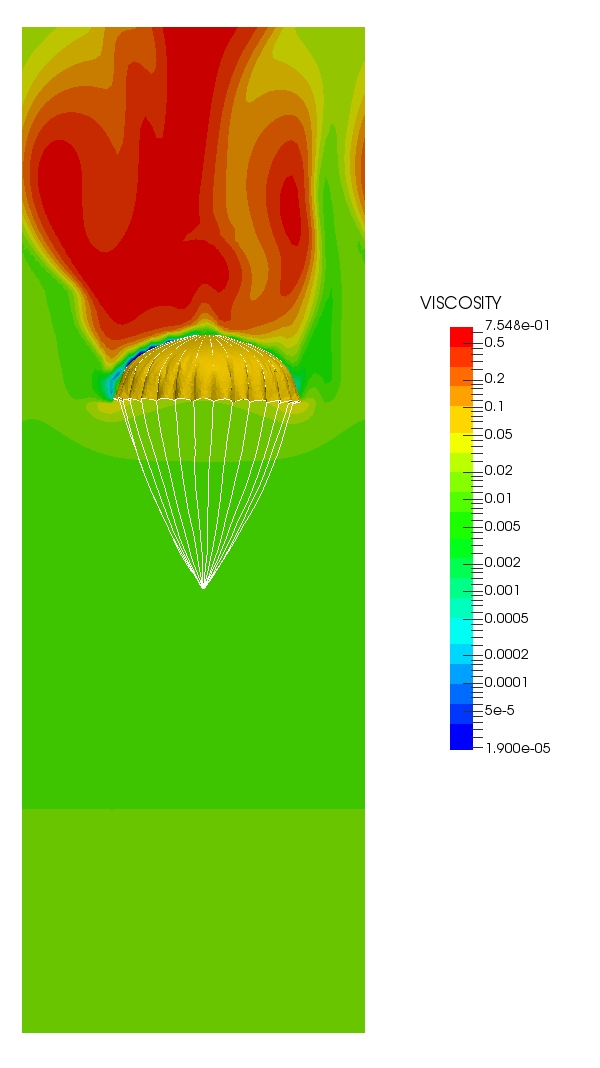
\includegraphics[width=0.24\textwidth]{Figures/c9-vis-std-15ms.jpg}
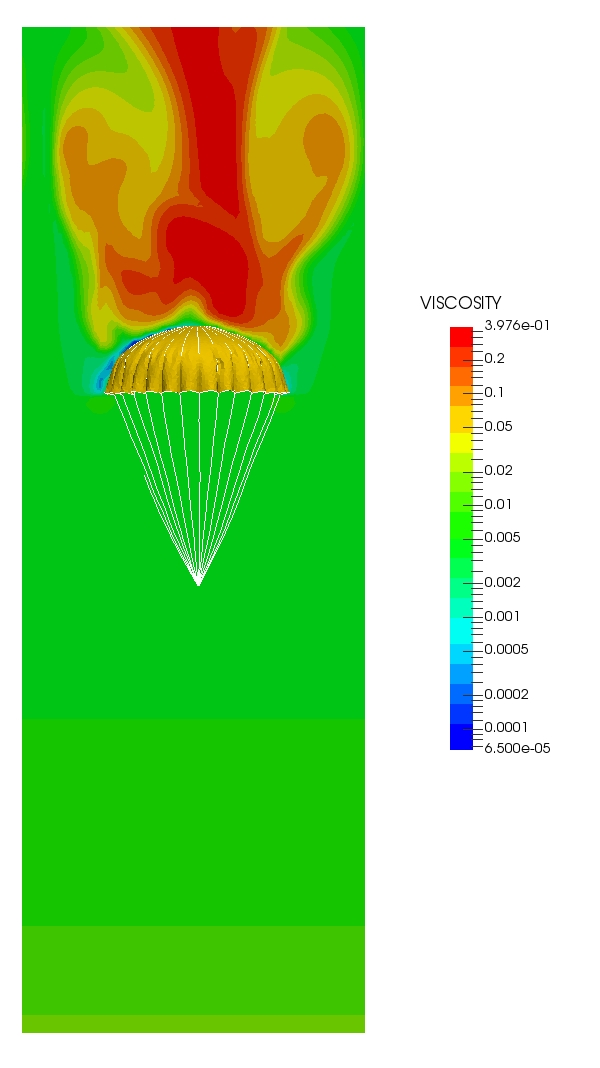
\includegraphics[width=0.24\textwidth]{Figures/c9-vis-rng-15ms.jpg}
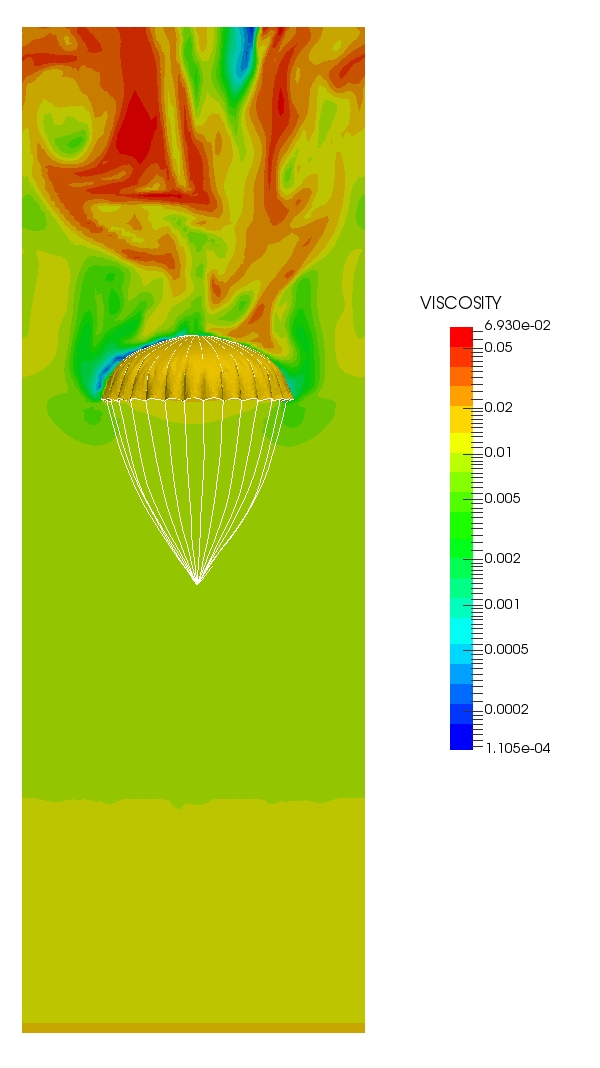
\includegraphics[width=0.24\textwidth]{Figures/c9-vis-real-15ms.jpg}
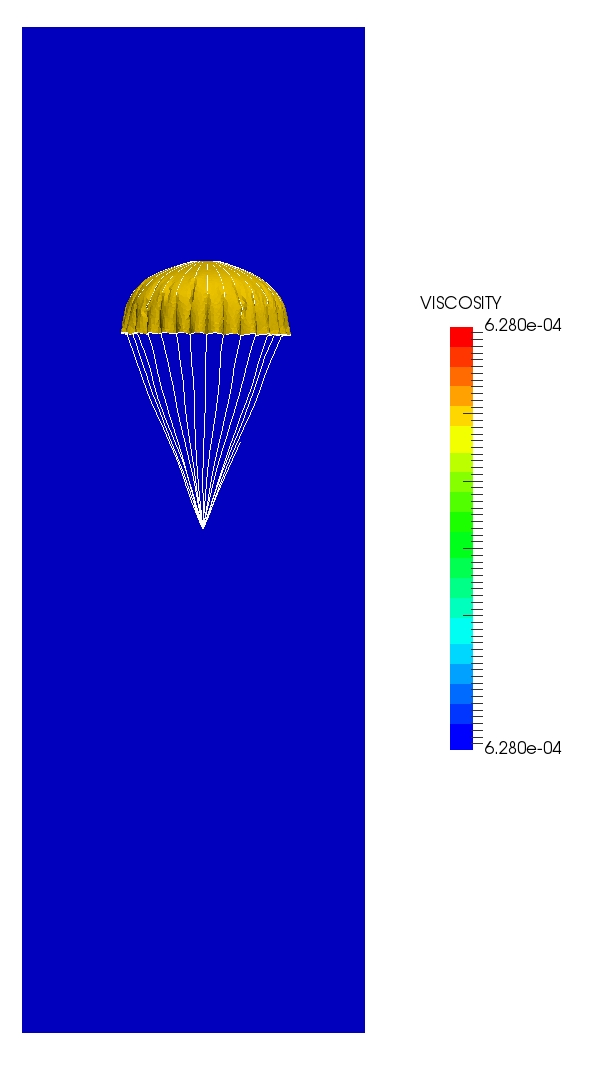
\includegraphics[width=0.24\textwidth]{Figures/c9-vis-lam-15ms.jpg}
\caption{Velocity magnitude and turbulent viscosity for C-$9$ parachute using different turbulent models at the same time frame. The inlet velocity is $15m/s$. The figures in the upper row displays the velocity magnitude and the figures in the lower row shows the turbulent viscosity.}
\label{turbulent_visc_vel_15ms}
\end{figure}
\subsection{Porosity model}
Two sets of numerical tests are carried out to validate the porosity model 
and its underlying numerical method. 
The first set of tests is designed to study a steady incompressible flow
through a porous interface. The purpose of this numerical test is to 
verify the implementation of our method. The pressure drop is expected to appear exactly 
at the interface position as the model described in \Eq{jumpcond}. 
The computational domain is set to be $4 m\times
0.4 m\times 0.4 m$ in the $x$, $y$, $z$ directions, respectively. The velocity is
driven by an inflow with a parabolic profile: 
\begin{equation}
\mathbf{u}(x=0,y,z) = [16U_{max}yz(L_y - y)(L_z - z)/(L^2_yL^2_z),0,0]
\end{equation} 
where $U_{max}$ is the maximum velocity at the center of the
inlet, $L_y$ and $L_z$ are the width of the channel in $y$ and $z$ directions. 
An outflow boundary condition together with the pressure $p = 0 Pa$ is applied to 
the outlet at $x = 4 m$ and a non-slip boundary condition of $\mathbf{u} = \mathbf{0}$ 
is imposed for the remaining faces. The porous interface is orthogonal to the streamline 
of flow and is placed at $x = 2m$. The coefficients in equation \Eq{jumpcond} are set as 
$\alpha = 10 kgm^{-1}s^{-1}$ and $\beta = 0 kgm^{-2}$.
The profiles of velocity and pressure at different positions are shown in \Fig{fig:test1_profile}.  	

\begin{figure}[H] \centering
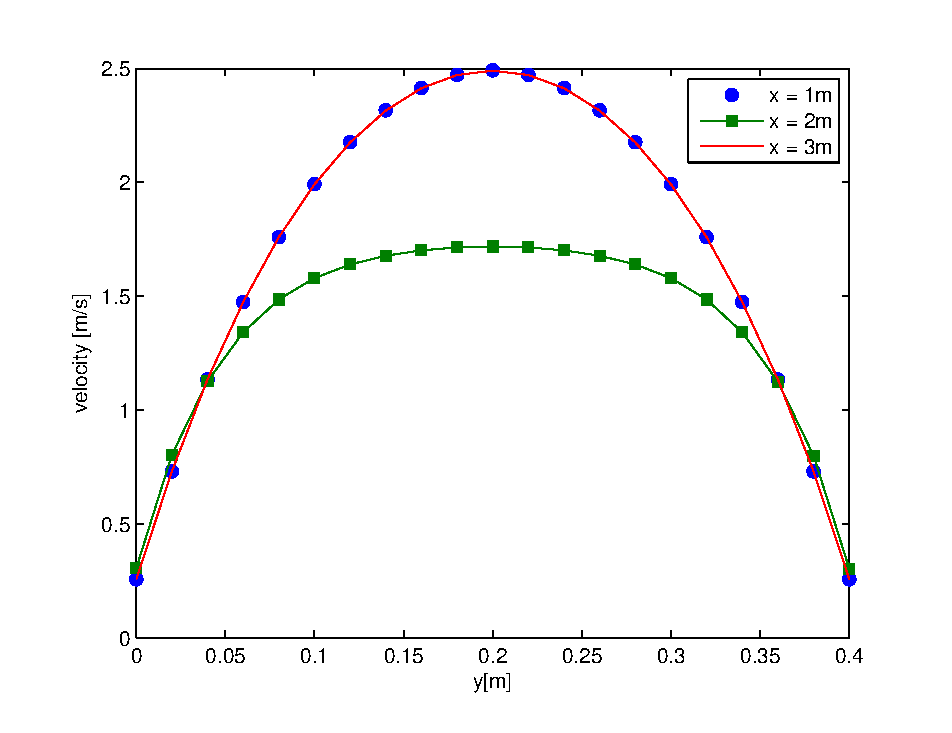
\includegraphics[width=0.49\columnwidth]{Figures/ucrs_profile}
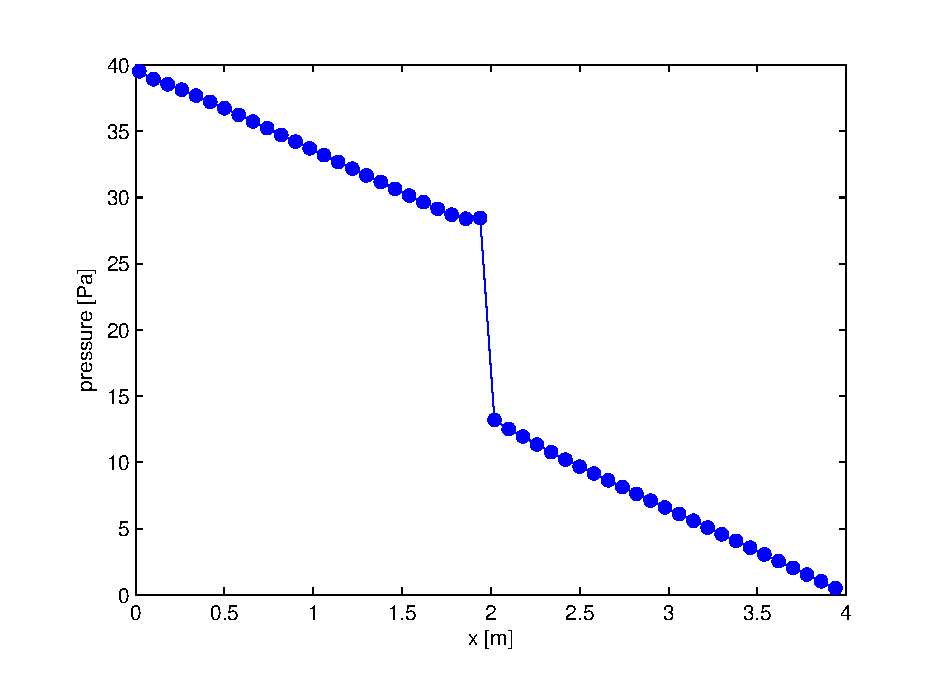
\includegraphics[width=0.49\columnwidth]{Figures/p_profile} \caption{(left)
Streamwise velocity profile at different sliced cross section and 
(right) pressure along a axial direction with $y = 0.2 m, z = 0.2 m$. The plot 
shows the velocity changes its profile as the fluid passes through the interface. 
The pressure drop at the interface is well captured.} 
\label{fig:test1_profile} 
\end{figure}

In the second set of tests, a full-scale model is used to simulate the response
of a realistic fabric surface in the channel flow.  The boundary conditions of
the computational domain are the same as the ones in the first test except that
the domain size is $30 m\times 10 m\times 10 m$. The elastic fabric surface located
at $x = 5 m$ is from the spring-mass model described in
\cite{Shi2015Verification}. Thus the surface can be stretched or compressed due
to the pressure drop at the interface.  The fabric tested in the simulations
resembles the properties of MIL-C-7020 type III fabric \cite{ewing1978recovery}
with density $533.77 kgm^{-3}$, Young's modulus $0.4309 Gpa$. The values of viscous 
and inertial parameters are $\alpha = 162 kgm^{-1}s^{-1}$ and 
$\beta = 48.82 kgm^{-2}$, which are calculated by fitting 
the experimental data using a quadratic function.
The permeability velocity and the pressure drop are 
measured by taking the average of the velocity and pressure drop over the entire surface. 
By imposing different values of inflow velocity, the functional relationship 
between these two variables can be obtained. We approximate the experimental data in \cite{ewing1978recovery} with formula $[p]_{\Gamma} = \alpha U_n + \beta U_n^2$ 
and use it as the reference solution. The results presented in \Fig{fig:curve} 
show that our model can successfully reproduce the quadratic relationship observed in the experiments. 

\begin{figure}[!htbp] \centering
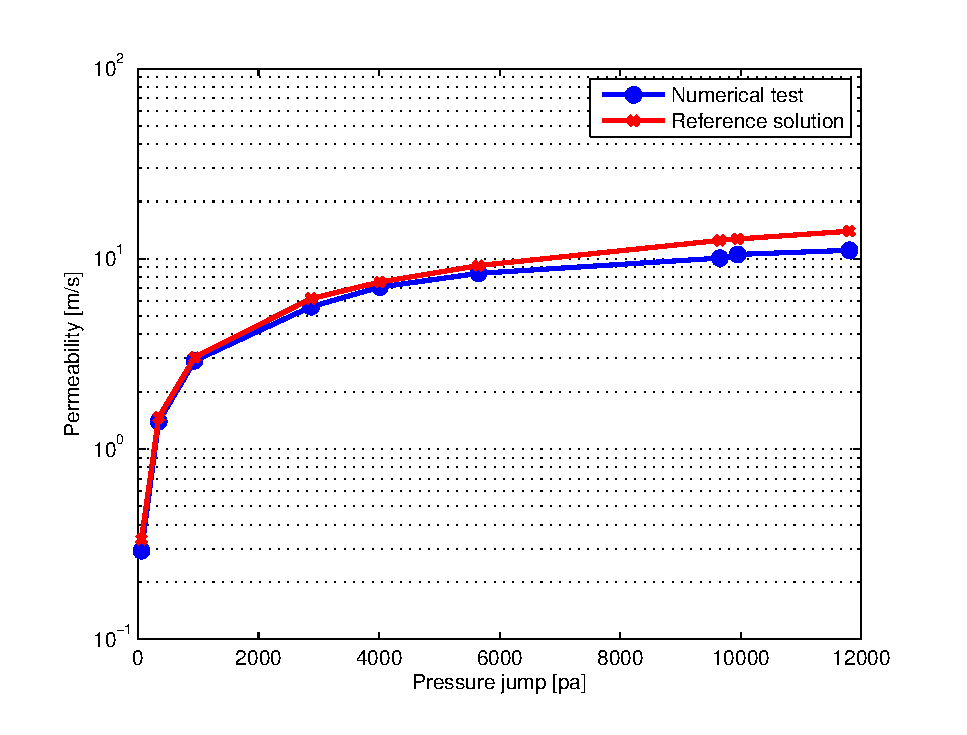
\includegraphics[width=1.0\columnwidth]{Figures/curve} \caption{Plot 
of permeability velocity vs. pressure drop for the test case. 
The numerical results show that there 
is a quadratic relationship between the permeability velocity and
pressure drop. Such relationship is observed in the experiment (red line)} 
\label{fig:curve} \end{figure}

In this section, we report our application of
the porosity model to the parachute simulation and compare the drag force with 
the same force as in the impermeable cases. The drag forces and drag
coefficients are calculated with varying freestream velocity at the inlet.
The drag measurement is carried out in a wind tunnel setting on G11 cargo
parachute with its nominal diameter $10 m$ and point of load fixed. The computational  
domain is set to be $14 m\times14 m\times40 m$ with constant velocity at the inlet, 
outflow boundary condition with pressure $p = 0 Pa$ at the outlet and periodic boundary 
condition for the rest of faces. The shapes of the parachute at different times are 
displayed in \Fig{fig:drag_test}. First, The parachute canopy is inflated by the 
inflow air. It then oscillates for a few seconds due to the elasticity of the string and the 
canopy, a process that is called parachute breathing \cite{roberts1974axisymmetric}. 
Eventually, it relaxes to a steady state shape due to damping friction force.

\begin{figure}[!htbp] \centering
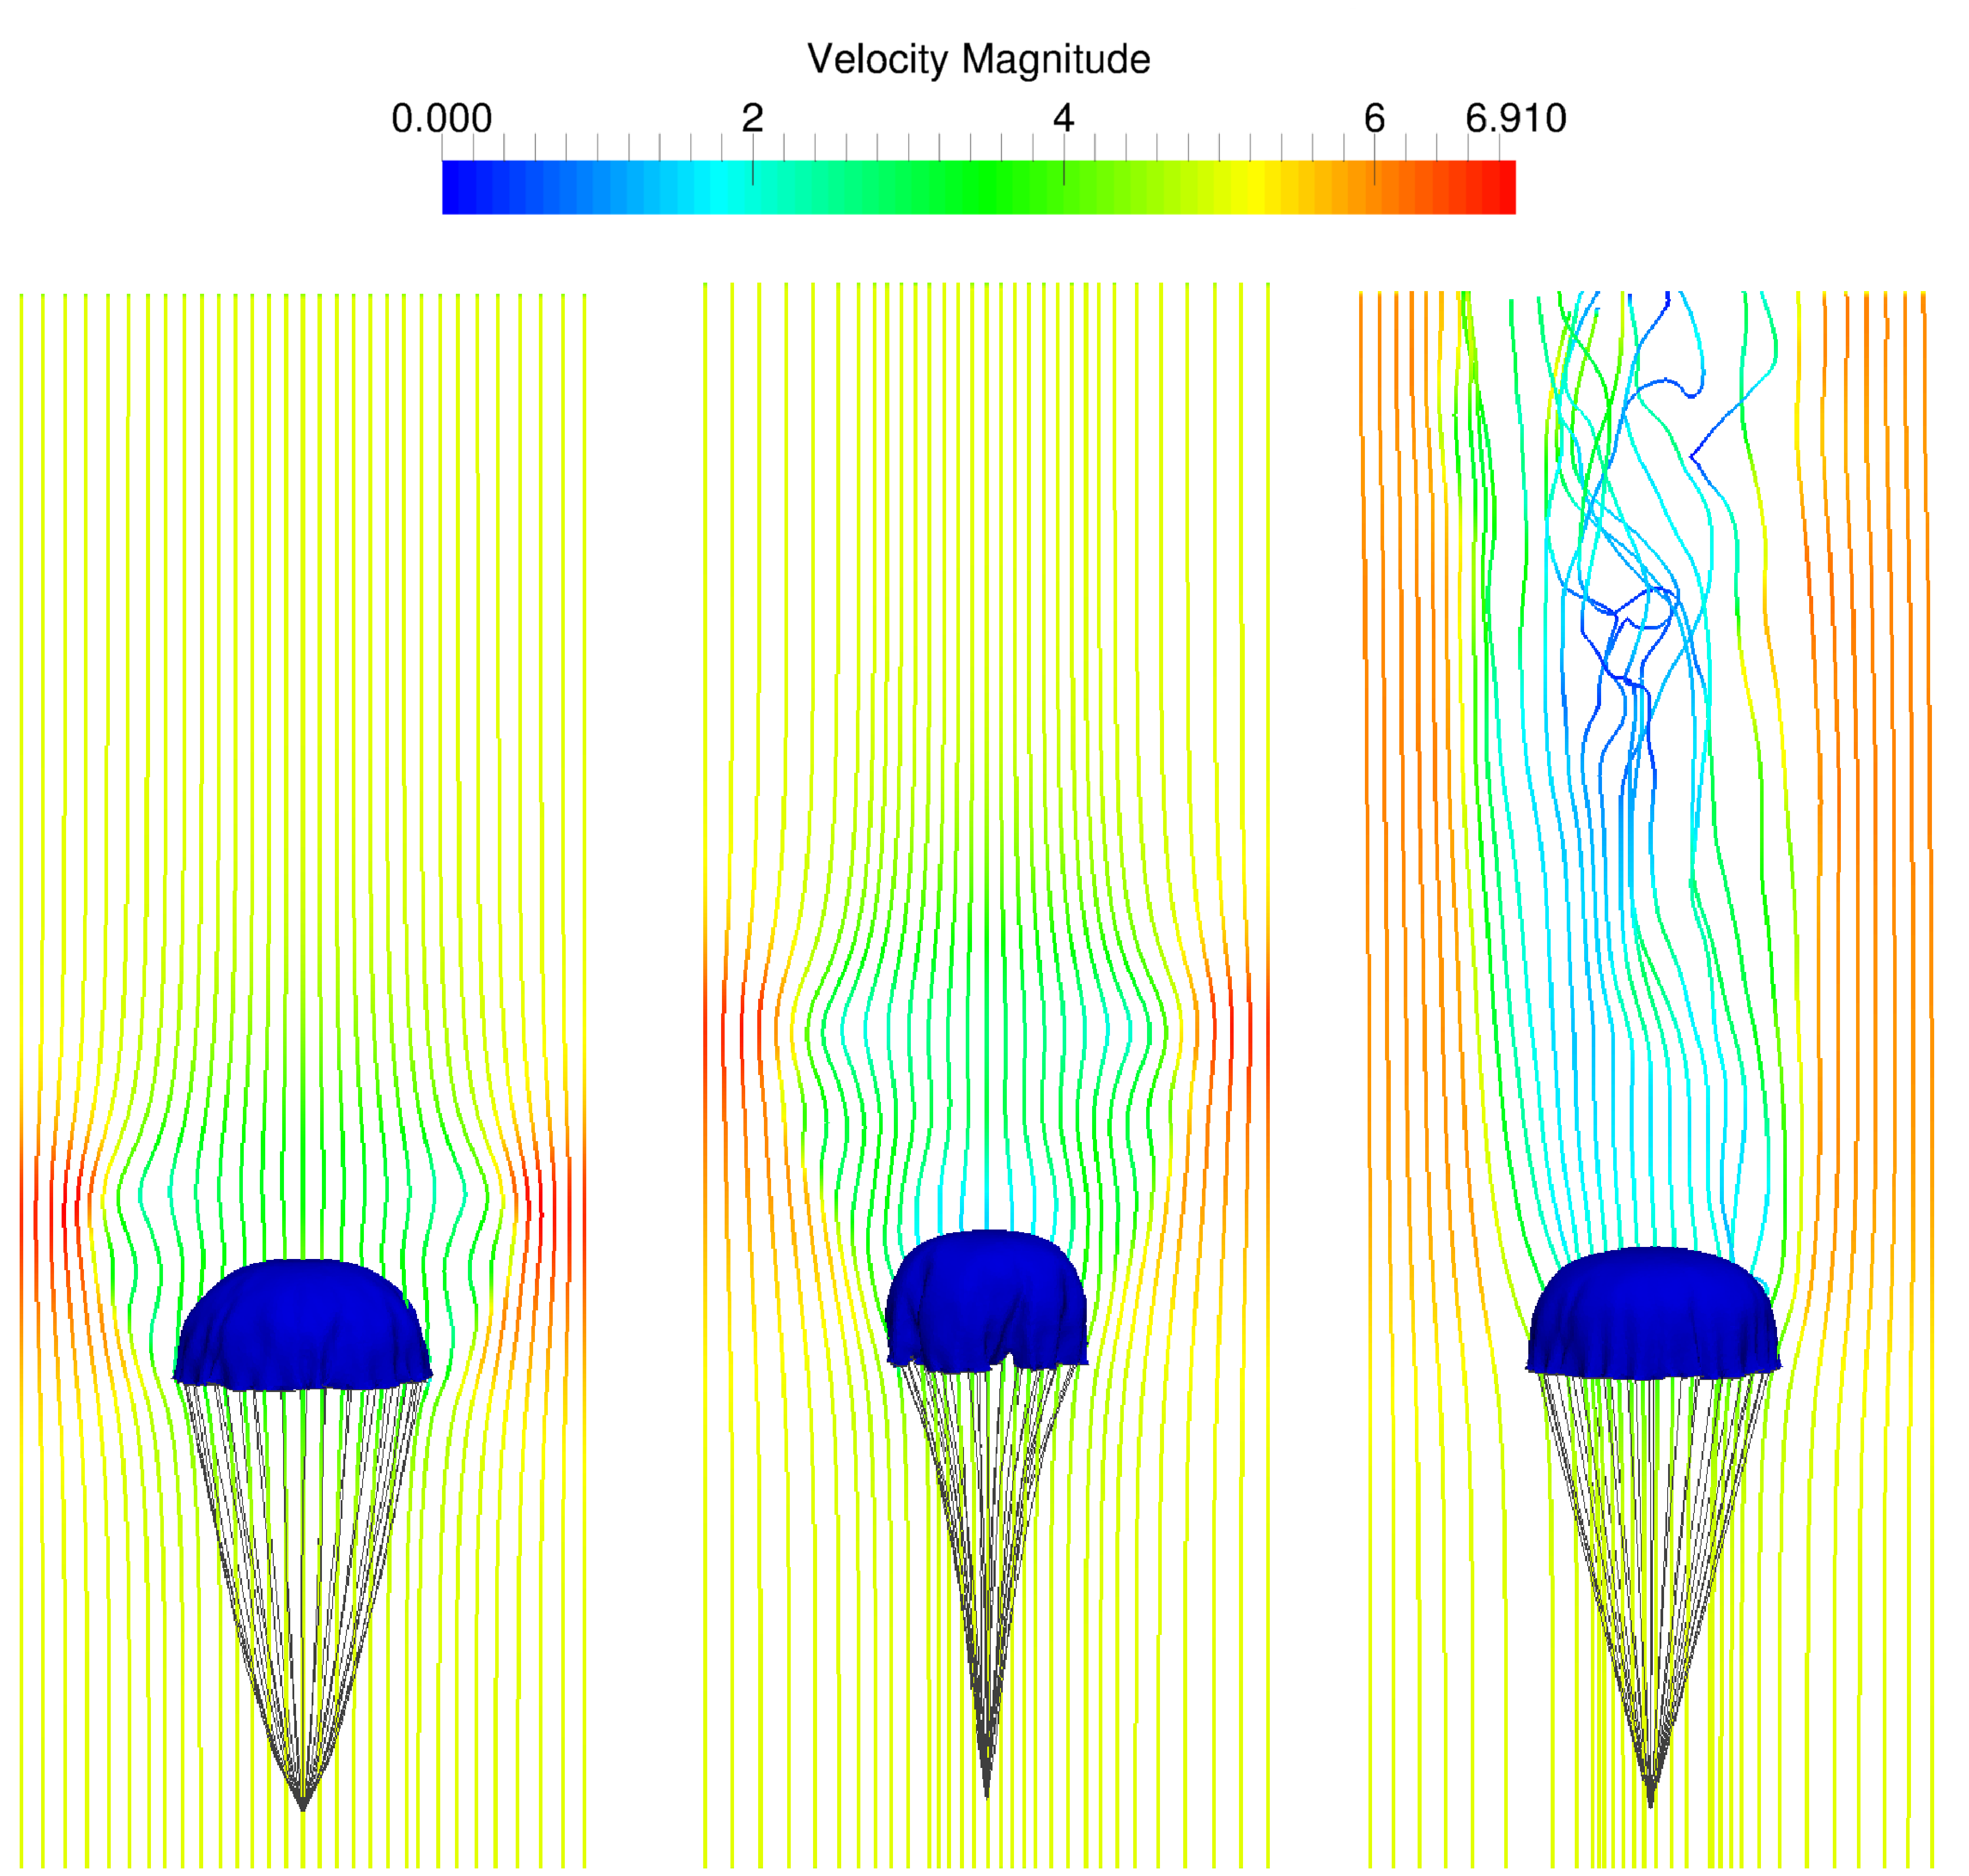
\includegraphics[width= 1.0\columnwidth]{Figures/drag_test} 
\caption{G11 cargo parachute in a numerical wind tunnel test
with the inlet velocity $5m/s$. The three plots from left to right are
the parachute shapes and velocity streamlines at 
the times $1.5s$, $2.5s$, and $15s$, respectively. The porosity 
coefficients in this case are set to be $\alpha = 6.7kgm^{-1}s^{-1}$, 
and $\beta = 3.1kgm^{-2}$. The oscillation of 
parachute canopy (parachute breathing) due to the elasticity of the parachute
string and the canopy is observed during the initial a few seconds. 
The streamlines are plotted with color 
to show the velocity magnitude.}
\label{fig:drag_test} \end{figure}

The drag force on the parachute is calculated by firstly integrating 
the pressure difference over all the surface elements (triangles) of the canopy 
and then projecting to the direction of the freestream velocity. After recording 
the drag force, the drag coefficient is calculated by the following formula: 
\begin{equation} 
C_d = \frac{F_d}{0.5\rho v^2_0A_0}
\label{eq:drag_coeff} 
\end{equation} 
where $\rho$ is the air density $= 1.2kg/m^3$, $v_0$ is the freestream velocity 
at the channel inlet and $A_0 = 78.5m^2$ is the area of parachute canopy at initial 
state. $F_d$ is the mean value of the drag force during the last $1s$ of the 
simulation. We observed that the drag coefficient increases at low descent velocities 
as displayed in \Table{table:drag_coeff}. This can be explained by the fact that the drag 
force (or the pressure drop) increases linearly at a very small velocity according to 
Ergun's equation, while the denominator has a quadratic growth.  

\begin{table}[H]
\centering
\begin{tabular}{cc}
\hline\hline
Inlet velocity ($m/s$) & Drag coefficients \\
\hline
$1.0$   & $1.89$ \\ 
$2.5$ & $1.31$ \\
$5.0$   & $0.92$ \\
$7.5$ & $0.63$ \\
$10.0$  & $0.49$\\
\hline
\end{tabular}
\caption{Drag measurements of the G11 parachute in wind tunnel tests
with varying inlet velocity and fixed the porosity coefficients 
$\alpha = 6.7kgm^{-1}s^{-1}$, $\beta = 3.1kgm^{-2}$.  
The drag coefficient decreases as the inlet velocity increases.}
\label{table:drag_coeff} \end{table}

To study the effects of the porosity on the parachute system,
we fix the inlet velocity at $3m/s$ while gradually increasing the
permeability of the parachute canopy. Although the porosity 
is not explicitly defined in our model, its relationship with the
parameters $\alpha$ and $\beta$ can be obtained
from the Ergun theory \cite{tutt2010development}:
\begin{equation}
\alpha = \frac{150\mu(1-\gamma)^2}{D^2\gamma^3}e, ~~~~
\beta  = \frac{1.75\rho(1-\gamma)}{D\gamma^3}e,
\end{equation}
where $\mu$ is the dynamic viscosity, $\rho$ is the density
of the air, $\gamma$ is the porosity of the parachute canopy,
$D$ is the characteristic length and $e$ is the thickness of the
porous surface. The porosity is defined 
as the fraction of the volume of voids over the total volume \cite{tutt2010development}.
Since the porosity is proportional to
$(\alpha/\beta^2)^{1/3}$, we can use the quantity  $(\alpha/\beta^2)^{1/3}$
instead of $\gamma$ to characterize the permeability of the
parachute canopy for our model. In fact, the parachute system is
affected by the porosity through in two ways. On one hand, the
porosity model will reduce the drag force on the parachute surface
by lowering the pressure difference. Since the viscous 
drag is ignored here, the pressure drag becomes the driving force affecting 
the shape and behaviors of the parachute.
On the other hand, the permeability
of parachute canopy could significantly affect the aerodynamic
field variables of the surrounding fluid such as pressure, flow velocity
and vorticity. These, in turn, will impact the stability of the
parachute system.

Another observation is that the parachute system would be more stable with
finite porosity than that of solely impermeable fabric.  This is shown by
comparing the drag force on the parachutes with and without fabric permeability
(see \Fig{fig:compare}).  

\begin{figure}[!htbp] \centering
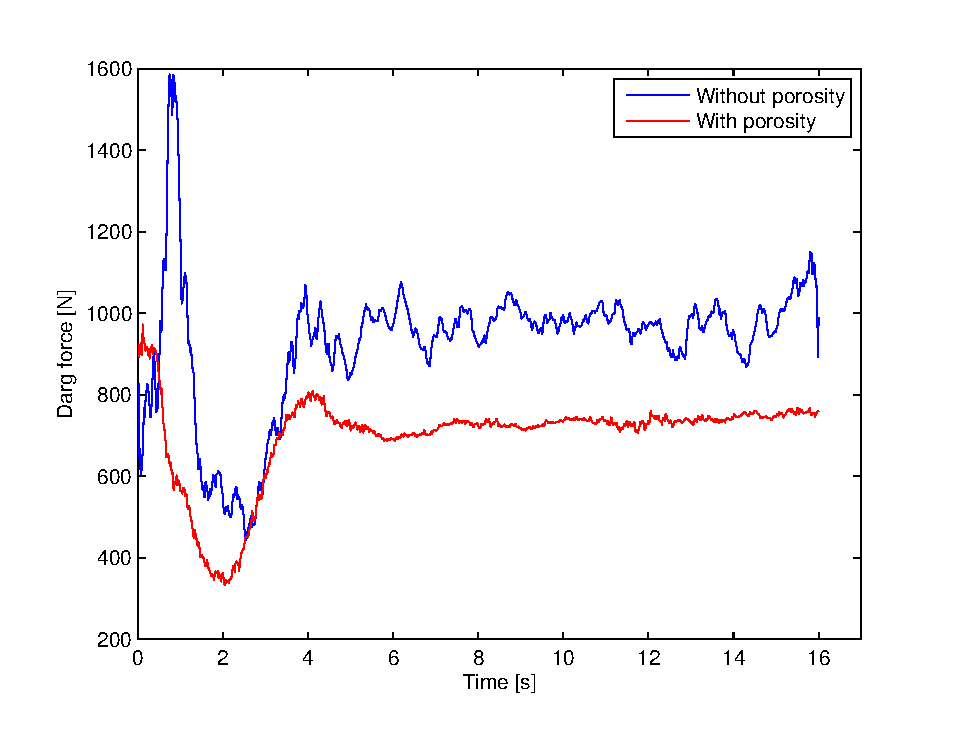
\includegraphics[width=1.0\columnwidth]{Figures/drag_compare} 
\caption{
Comparison of drag force for G11 parachute between the permeable (red) and 
impermeable (blue) canopies in the same simulation. The porosity coefficients 
are set to be $\alpha = 6.7kgm^{-1}s^{-1}$, $\beta = 3.1kgm^{-2}$. 
The increase of porosity leads to the reduction of drag force 
and the vorticity in the wake of the canopy, thus make the drag force
less oscillatory.} 
\label{fig:compare} 
\end{figure}

\subsection{Collision handling and folding algorithm}
In this section, the results of collision detection, collision handling, and 
folding algorithm are presented. Firstly, we have tested the performance of 
the collision handling algorithm. Several benchmark tests have been carried 
out: a round fabric falling on a rigid box; a round fabric falling on strings. 
These tests demonstrate the capability 
of our algorithm that can universally handle the interactions between fabric 
surface, rigid bodies and strings. \Fig{fig:collision_test} shows that the 
collision algorithm can produce visually plausible results and successfully 
eliminate all the intersections in the fabric. 
\begin{figure}[!htbp]
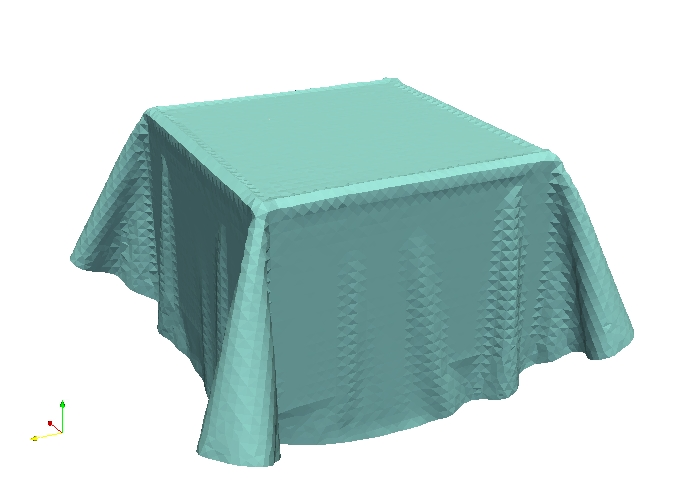
\includegraphics[width=0.45\columnwidth]{Figures/fabric-box.jpg}
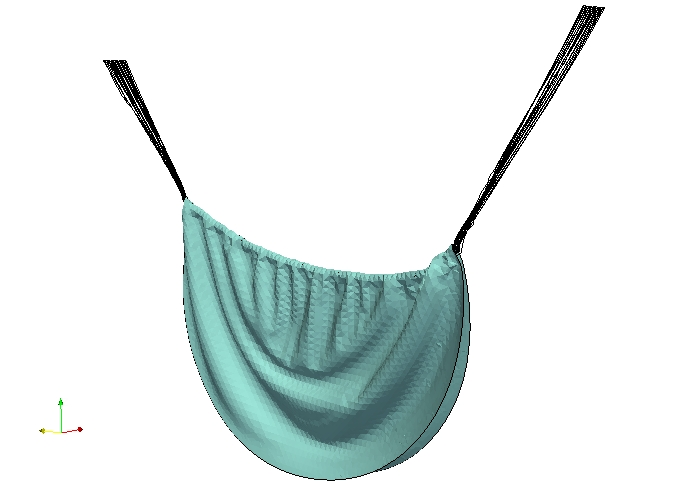
\includegraphics[width=0.45\columnwidth]{Figures/fabric-string.jpg}
\caption{Benchmark test for collision detection and handling. Two cases are 
considered: interactions of fabric with rigid body (left) and elastic (right).
Note that the fabric's self-interactions are also handled well during the 
collision procedure.}
\label{fig:collision_test}
\end{figure}
In order to test the performance of 
the collision algorithm on a more complicated geometry, a simulation of a fabric
dropping from above of a rigid human model has been carried out. 
\Fig{fig:collision_test_human} displays three frames of the simulation and shows 
that the algorithm can well handle the collision between fabric and a non-trivial geometry.
\begin{figure}[!htbp]\centering
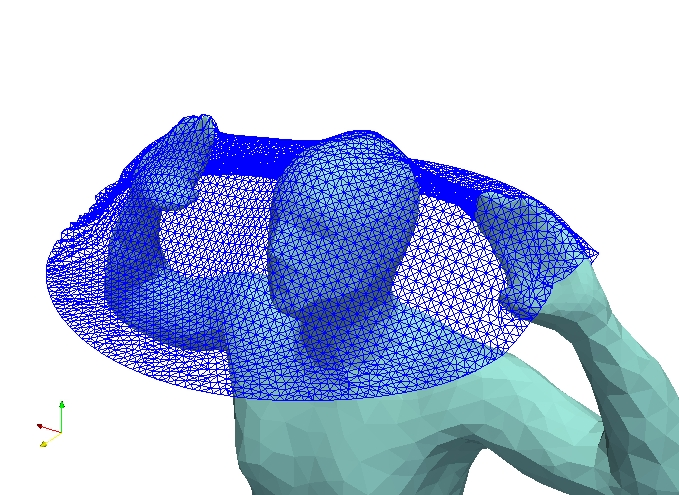
\includegraphics[width=0.3\columnwidth]{Figures/fabric-body-0.jpg}
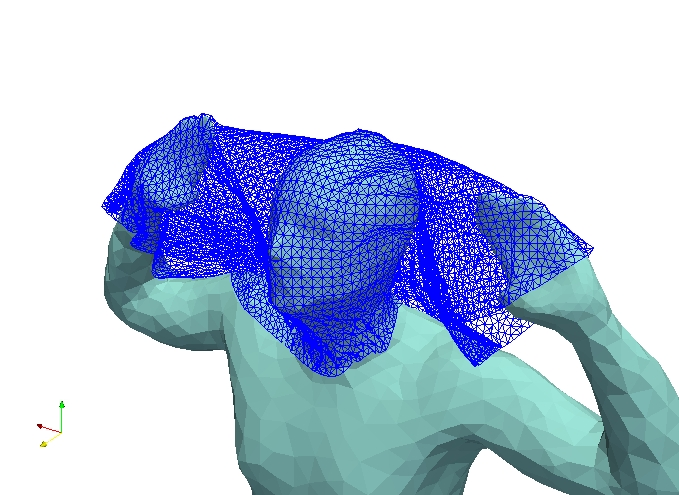
\includegraphics[width=0.3\columnwidth]{Figures/fabric-body-1.jpg}
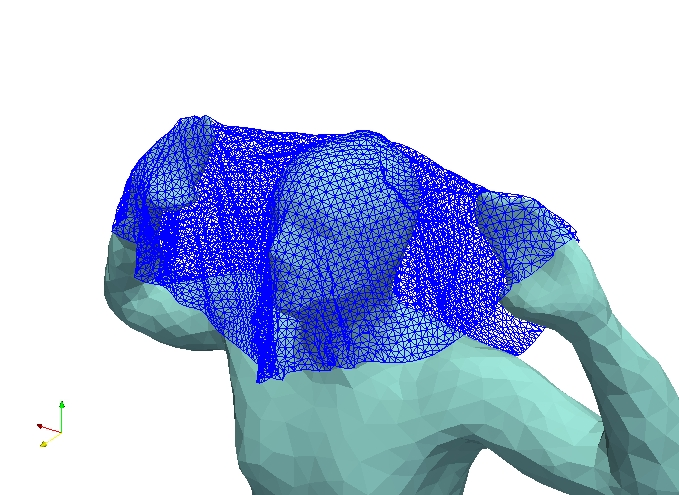
\includegraphics[width=0.3\columnwidth]{Figures/fabric-body-2.jpg}
\caption{Three movie frames in the simulation of collision between elastic fabric and rigid human model.}
\label{fig:collision_test_human}
\end{figure}

The folding algorithm is verified by close a round parachute canopy with $16$ creases. Here we name this folding pattern as ``close folding". Two groups of the folding angles are assigned corresponding to the mountain and valley crease alternatively. The final folding angle of the mountain crease is $-\pi$ and the folding angle of the valley crease is $3\pi/4$. The folding algorithm can automatically proceed and reach the desired state without any artificial controls. Three frames of the folding procedure are displayed in \Fig{fig:folding_para}. It can be seen that the canopy remains unstretched and the final state is perfectly symmetric. To explain the folding algorithm more clearly, the $16$ folding angles of the close folding are recorded and plotted in \Fig{fig:folding_angles}. The left panel is the behavior of the folding angles in the entire simulation and the right panel is a plot of the first $25$ steps. It is clear that the angles are moved randomly while gradually approach to the final state. This 
is because the optimization algorithm is based on a random search, and hence the folding angle can not be guaranteed to move uniformly. However, this behavior would not affect the eventually folded state, and in the meanwhile, the folding angles still strictly satisfy the necessary condition of the origami design. In conclusion, this folding algorithm provides a highly flexible and universal way to design various folding patterns. Only the folding angles and creases pattern are required as inputs while the intermediate folding process is completely automatic.
\begin{figure}[!htbp]\centering
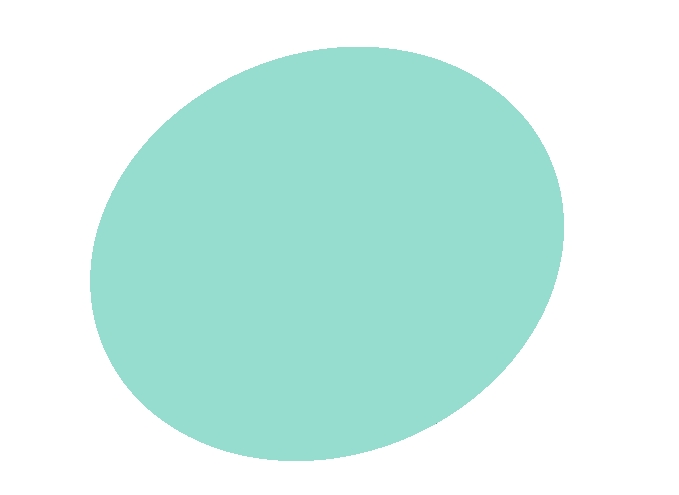
\includegraphics[width=0.3\columnwidth]{Figures/fold-0.jpg}
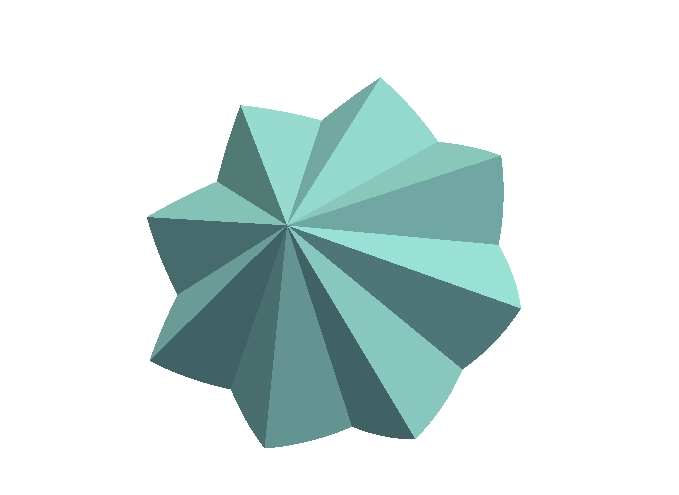
\includegraphics[width=0.3\columnwidth]{Figures/fold-1.jpg}
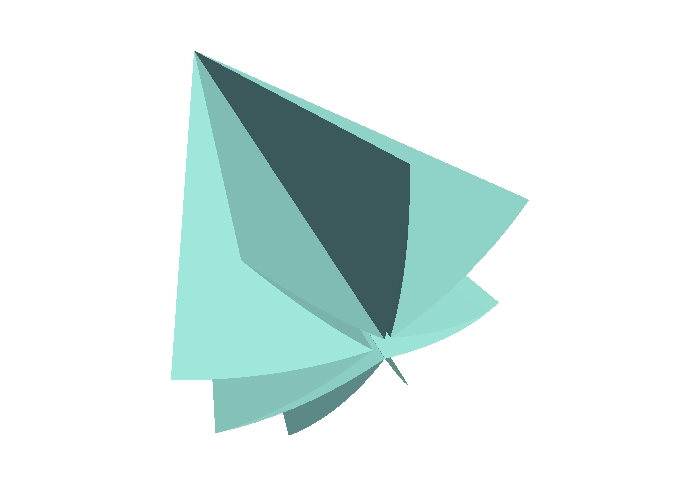
\includegraphics[width=0.3\columnwidth]{Figures/fold-2.jpg}\\
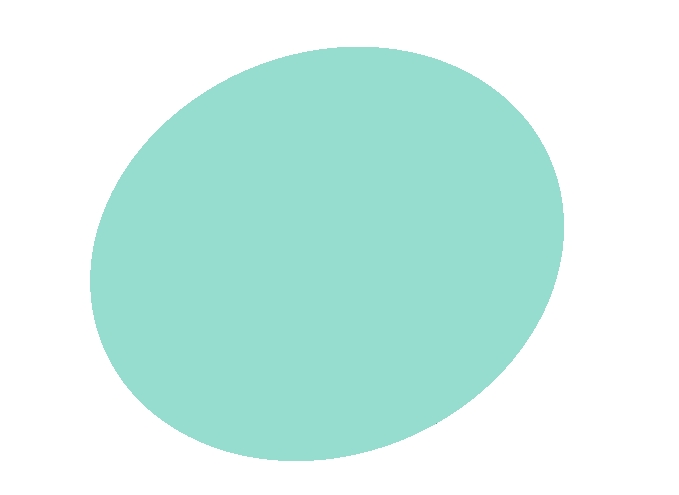
\includegraphics[width=0.3\columnwidth]{Figures/fold-0.jpg}
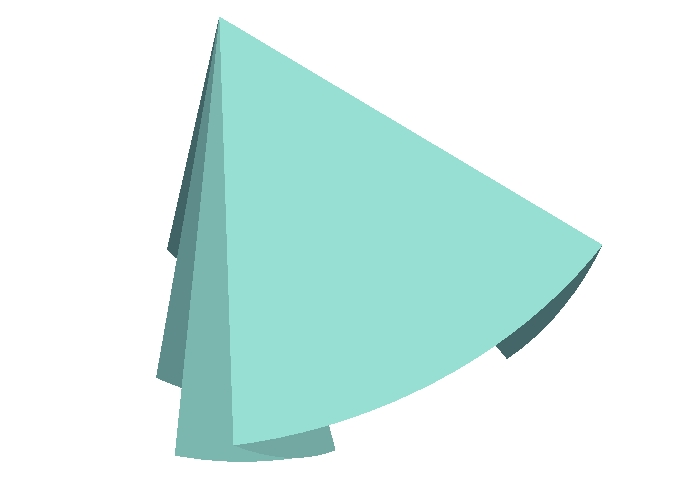
\includegraphics[width=0.3\columnwidth]{Figures/fold-flat-1.jpg}
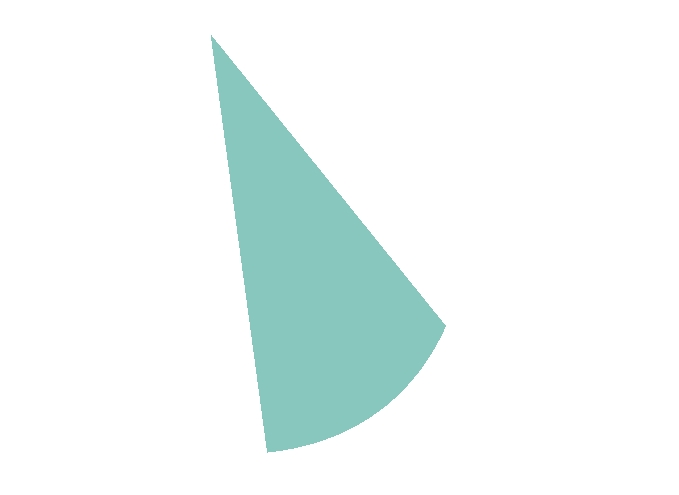
\includegraphics[width=0.3\columnwidth]{Figures/fold-flat-2.jpg}
\caption{Three movie frames of the parachute canopy shape in the folding process. The upper panel displays the close of a parachute canopy and the lower panel displays the flat fold.}
\label{fig:folding_para}
\end{figure}

\begin{figure}[!htbp]\centering
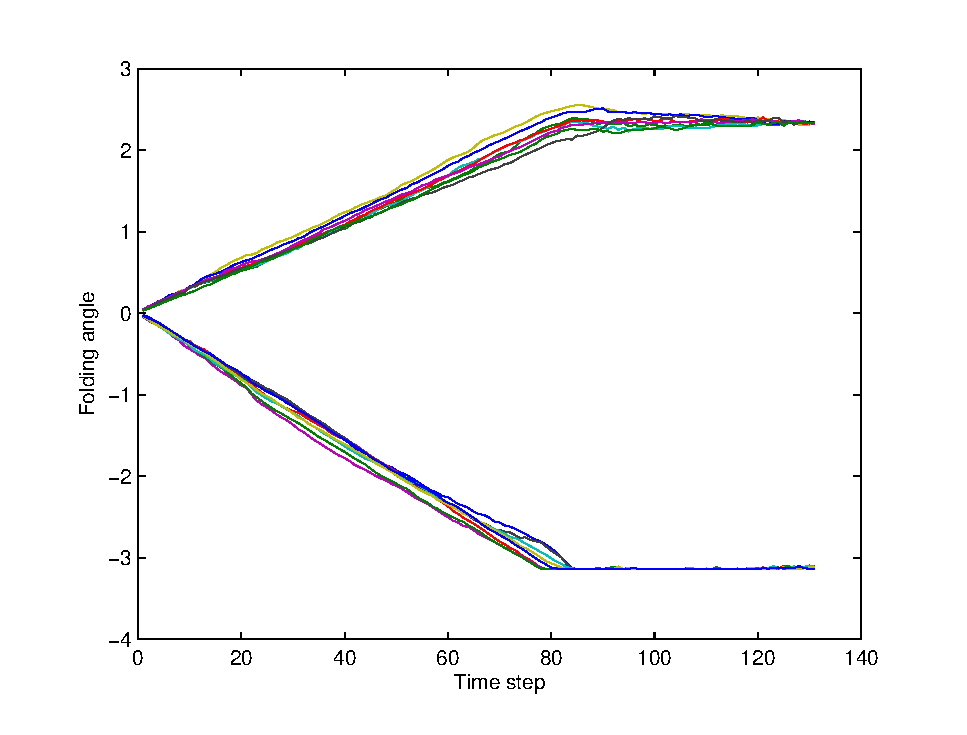
\includegraphics[width=0.45\columnwidth]{Figures/folding-angle}
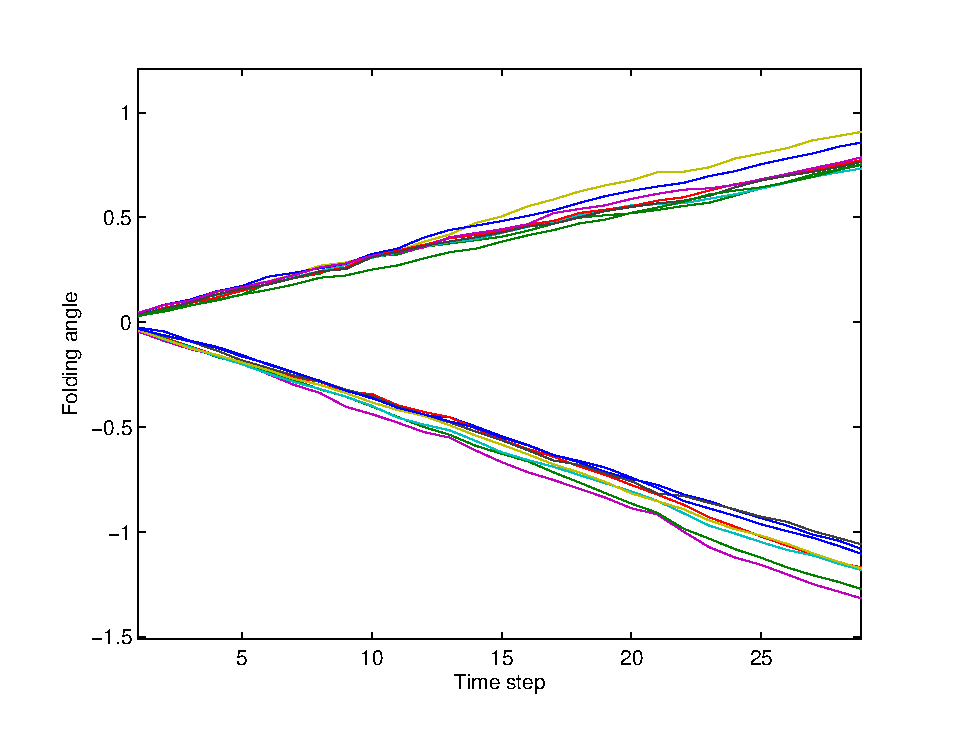
\includegraphics[width=0.45\columnwidth]{Figures/folding-angle-zoom}
\caption{Folding angles of the $16$ creases. Right panel shows the magnification of the irst $25$ steps.}
\label{fig:folding_angles}
\end{figure}

\section{Results for cloud entrainment and mixing}

\subsection{Initial conditions}   
%Following quantities are defined to characterize the turbulence field. 
%The dissipation rate is defined as $\epsilon=2\nu\langle (\nabla\times \mathbf{u})^2)\rangle$,
%$\nu$ is the kinematic viscosity of air $1.5\times10^{-5}m^{2}s^{-1}$, and $u_{rms}$
%is the root mean square of velocity fluctuation. $\tau_{\eta}$ is
%the Kolmogorov time scale defined as $(\nu/\epsilon)^{1/2}$. $\tau_L$
%is the eddy turnover time, estimated by $L_x/u_{rms}$
%where $L_x$ is the domain size.

Three different initial configurations of cloudy area are used to investigate the impact of cloudy area configuration. Case 1 follows that used in \cite{And04} whereby water mixing ratio is defined according to the sign of the velocity function in physical space such that
\begin{equation}
\mbox{case 1: } q_v(\mathbf{x},t=0) = 
\left\{\begin{array}{lr}
q_v^{max}, & u(\mathbf{x}) > 0\\
q_{v,e}, & u(\mathbf{x}) \le 0
\end{array}\right.\label{case1}
\end{equation}
where $q_v^{max} = 3.95 g/kg$ is the maximum amplitude of $q_v$, which exceeds $q_{v,s}$ by $2\%$, and $q_{v,e} = 0.03g/kg$ is the vapor mixing ratio of the clear air. $u(\mathbf{x})$ is the first component of the fluid velocity. 

In \cite{Kumar11}, the author investigated a slab-like cloud configuration approximated with a smooth function to avoid the Gibbs phenomenon (numerical overshoots at sharp interfaces). Similarly, our Case 2 is designed to study the slab-like configuration but approximiated with a simple discontinuous function given by
\begin{equation}
\mbox{case 2: } q_v(x,t=0) = 
\left\{\begin{array}{lr}
q_v^{max}, & (L-d)/2 \le x < (L+d)/2\\
q_{v,e}, & \mbox{elsewhere}
\end{array}\right.\label{case2}
\end{equation}
where the $q_v^{max}$ and $q_{v,e}$ are the same as in Case 1.
$L$ is the length of computational domain, and $d = L/2$ is the width of the cloud slab.

It is well known that entrainment-mixing processes can also occur near cloud tops, esp., for stratiform clouds \cite{Lu2011, Yum2015}. To mimic the cloud-top entrainment-mixing process, herein we add a new cloud configuration by rotating Case 2 by $90$ degree, and name it Case 3.
\begin{equation}
\mbox{case 3: } q_v(z,t=0) = 
\left\{\begin{array}{lr}
q_v^{max}, & (L-d)/2 \le z < (L+d)/2\\
q_{v,e}, & \mbox{elsewhere}
\end{array}\right.\label{case3}
\end{equation}

The temperature field is initialized by imposing the neutral buoyancy condition \cite{Kumar14} such that:
\begin{equation}
T(x,t = 0) = T_0 - 0.608T_0[q_v(x,t = 0) - q_{v0}]
\end{equation}
where the reference values are defined by the domain averages $T_0 = \langle T(t=0)\rangle_V$ and $q_{v0} = \langle q_v(t=0)\rangle_V$. This neutral buoyancy condition ensures the initial cloudy area having higher water vapor mixing ratio but lower temperature compared to the environment. Note that this procedure is only performed for the initial temperature field; later temperature field completely follow \Eq{eq:Temp} afterwards. \Fig{fig:slice_case123} compares the initial fields of water vapor 
mixing ratio and temperature for the three cases. The discrepancies between the initial water vapor 
and temperature fields are self-evident, allowing for examination of the impacts of the initial 
configuration of cloudy area on entrainment-mixing processes. Note that all the three initial 
configurations have the same initial cloud fraction of $0.5$, and the same dynamical field.

\begin{figure*}\centering
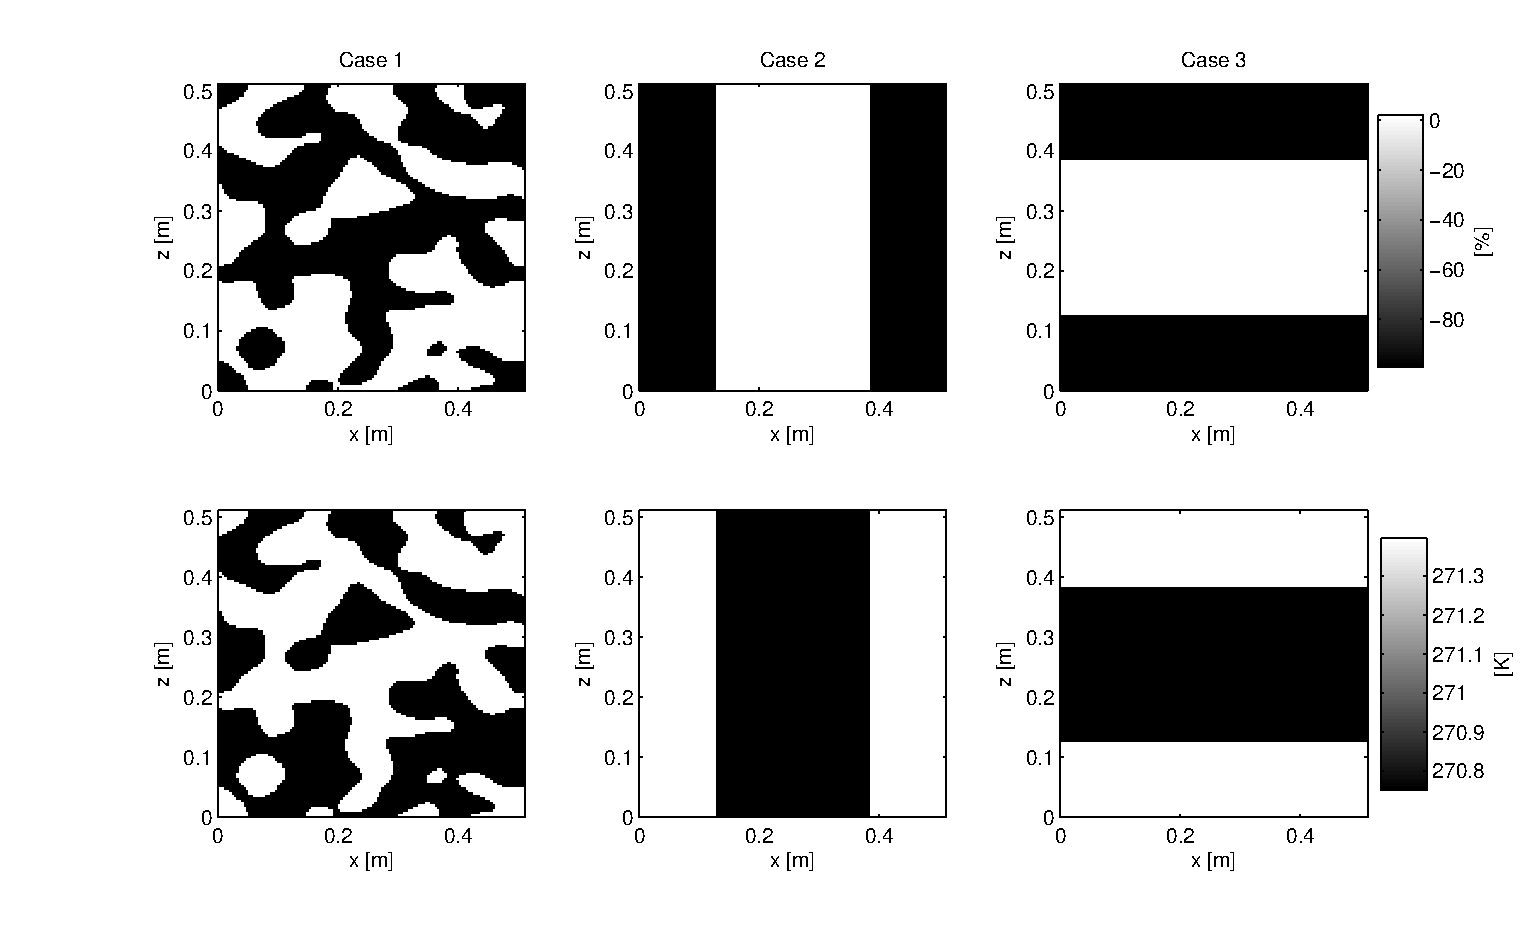
\includegraphics[width=0.9\linewidth]{Figures/init_vapor_supersat}
\caption{Cross sectional view of the initial supersaturation and temperature (K) field for different cases: case 1, 2, 3 from left to right. The cloudy part occupies about half of the computational domain.\label{fig:slice_case123}}
\end{figure*}

At beginning, a total of $10^{7}$ droplets with the same radius of $15\mu m$  are randomly placed in the cloudy area according to the Poisson point process, giving a droplet number concentration of $ ~ 153{cm}^{-3}$. Note that for the forced turbulence scenario, the velocity field needs a few steps ($5$ seconds here) to relax to a steady state. Therefore, the droplets are released to move and change their sizes according to the physics law after this spin-up period. For the decaying turbulence, the droplets are released at time $t = 0s$ since there is no needs to seek for a steady state. The simulation is terminated when droplets completely evaporate or the field becomes nearly uniform ($std < 0.0002$). 

For convenience, \Table{tb:parameters} summarizes the key quantities and initial conditions.
\begin{table}\centering
\resizebox{\textwidth}{!}{
\begin{tabular}{l c c c c c}
\hline\hline
Quantity & Symbol & Value & Quantity & Symbol & Value\\
\hline
Grid points & $N$ & $256$ & Droplet radius & $R_{0}$ & $15\mu m$\\
Box length & $L$ & $0.512m$ & Environ supersat & $S_{e}$ & $-99\%$\\
Grid size & $a$ & $0.002m$ & Cloud supersat & $S_{c}$ & $2\%$\\
Viscosity & $\nu$ & $1.5\times10^{-5}m^{2}s^{-1}$ & Number concentration& $N_{c}$ & $153cm^{-3}$\\
Dissip rate& $\epsilon$ & $2.0\times10^{-3}m^{2}s^{-3}$ & Eddy turnover time & $\tau_{L}$ & $4.27s$\\
Dissip length& $\eta$ & $10^{-3}m$ & Evaporation time & $\tau_{evap}$ & $2.09s$\\
Dissip time& $\tau_{\eta}$ & $0.087s$ & Reaction time & $\tau_{react}$ & $4.52s$\\
\hline
\end{tabular}}
\caption{Summary of key model parameters and initial conditions}
\label{tb:parameters}
\end{table}

\subsection{Dynamical fields and microphysics}
\Fig{fig:therm_dynam} compares the temporal evolutions of the domain mean, standard deviation and relative dispersion of turbulent kinetic energy (TKE, a, b, c), of temperature (d,e,f) and water vapor mixing ratio (g, h, i), and supersaturation (j, k, l) between the six scenarios.  As expected, the mean TKE and its standard deviation for the three forced simulations (F1, F2 and F3) remain approximately constant determined by the large scale forcing after a short relaxation at the initial time. However, it is interesting to observe a transient turbulence enhancement before gradually decaying to zero in the decaying cases, especially for D2 and D3. This transient enhancement likely results from the buoyancy effect, which is caused by the deviation of temperature and vapor mixing ratio to the reference value according to \Eq{eq:source_term}. The D3 simulation exhibits the strongest enhancement, followed by D2. But for D2 the enhancement lasts longer. The mixing in D3 is accelerated by the sedimentation effect, making it a slightly stronger and faster than D2. Note that D1 can be regarded as the intermediate stage of mixing process in D2 or D3, and therefore the buoyancy effect quickly disappear and show little enhancement in the figure.  Most of the droplets have a chance to enter into the clear air and evaporate at an early stage. Evaporation process absorbs latent heat from the environment, resulting in deviation of the temperature field from the mean value. The transient enhancement can be seen more clearly from the standard deviation of temperature. The transient enhancement is weaker for the three forced simulations F1, F2 and F3 (but still stronger than that of TKE).  It is noteworthy that the behavior of transient turbulence enhancement does not appear in the field of water vapor mixing ratio, which is consistent with \cite{Kumar14}. Notice that the vapor mixing ratio in the clear air is much lower than in the cloudy air. The droplets entering into the clear area will quickly turn into vapor while the droplets staying in the cloudy area continue to grow by condensation. This phase transition process reduces the difference of vapor mixing ratio between clear air and cloudy air, thus the transient growth of the deviation can hardly be observed.  The behavior of supersaturation reflects the combination of temperature and water vapor mixing ratio, as expected. The variations manifest themselves in the plots of relative dispersion defined as standard deviation to the mean of the corresponding variables.

\begin{figure*}[!htbp]\centering
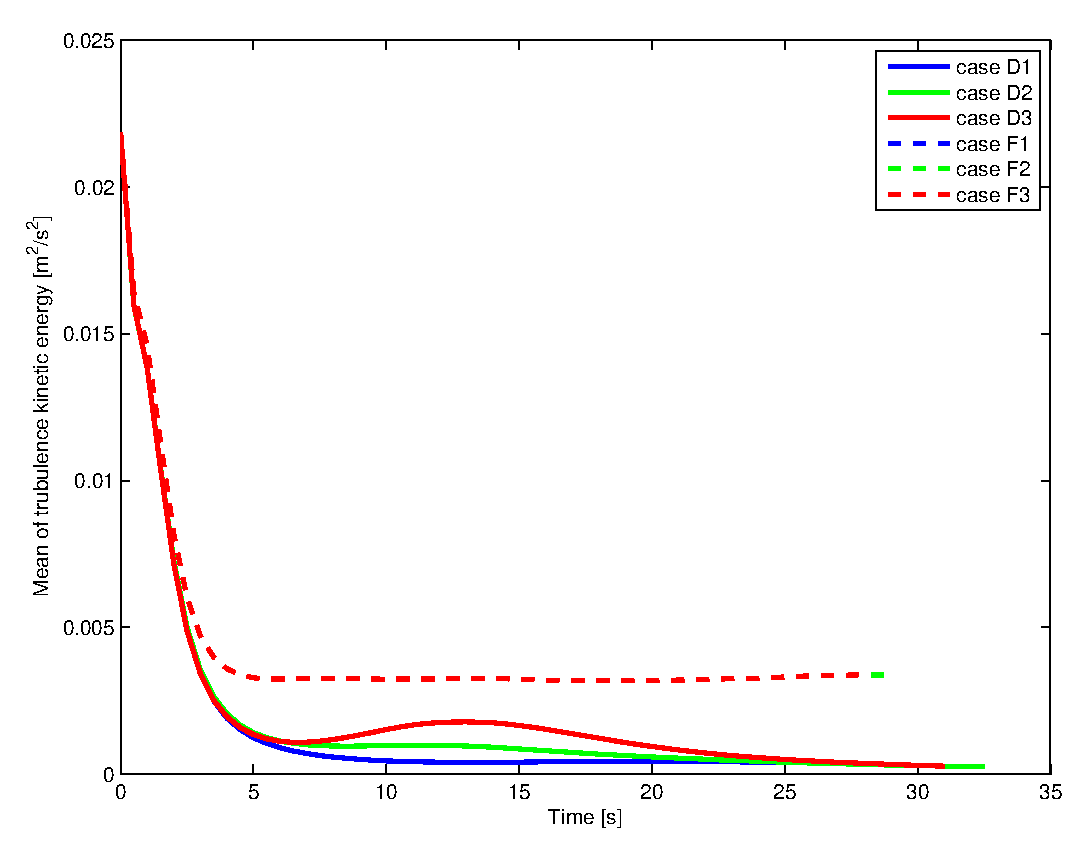
\includegraphics[width=0.3\linewidth]{Figures/mean_tke}
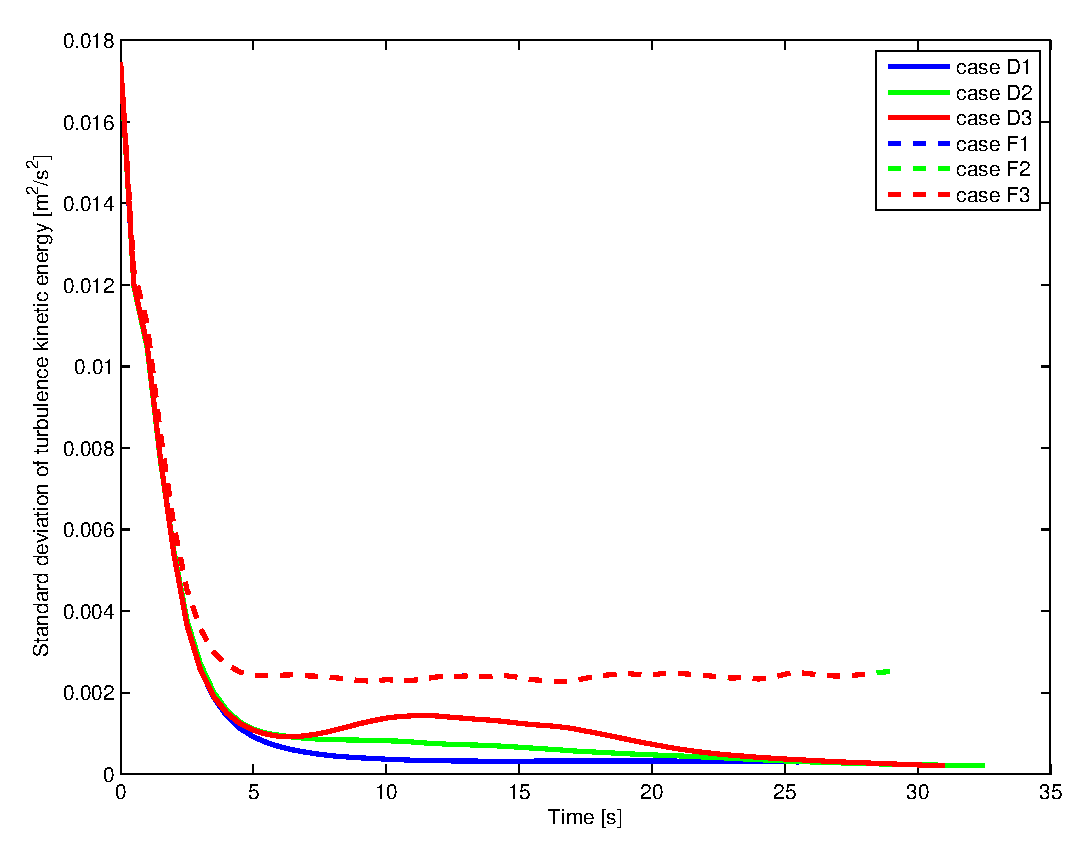
\includegraphics[width=0.3\linewidth]{Figures/std_tke}
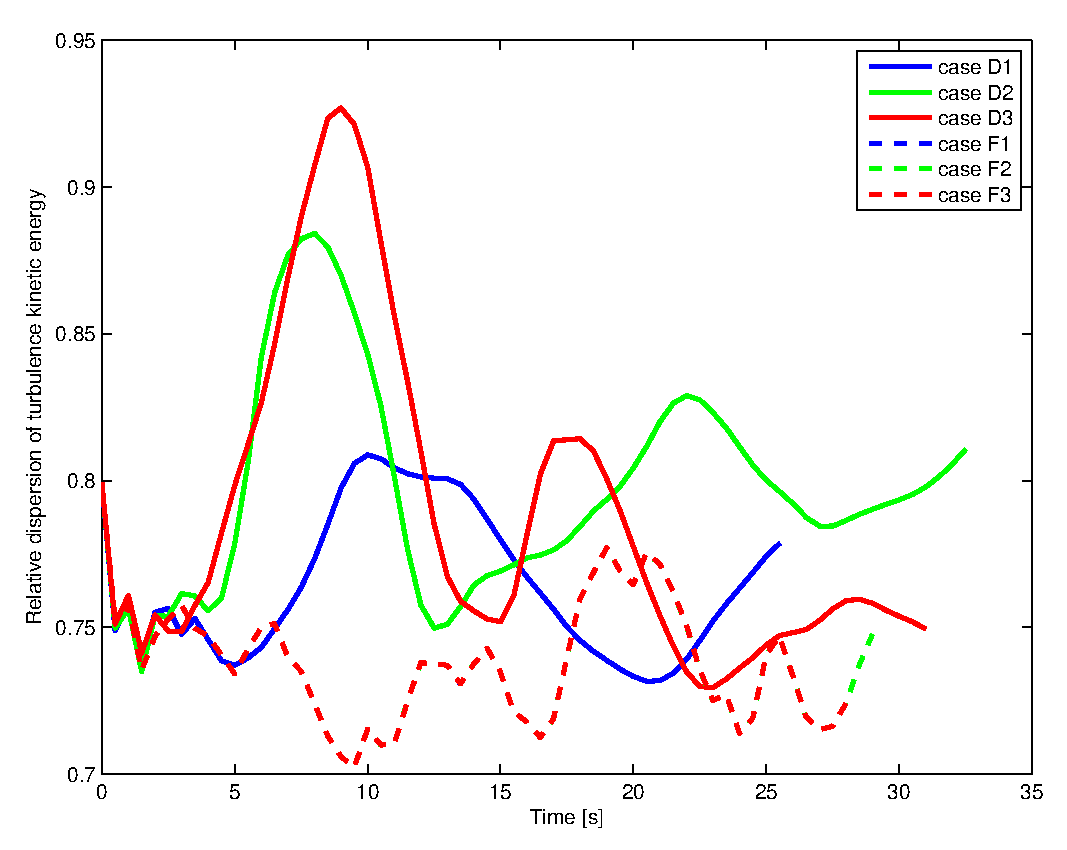
\includegraphics[width=0.3\linewidth]{Figures/dsp_tke}\\
\includegraphics[width=0.3\linewidth]{Figures/mean_temp}
\includegraphics[width=0.3\linewidth]{Figures/std_temp}
\includegraphics[width=0.3\linewidth]{Figures/dsp_temp}\\
\includegraphics[width=0.3\linewidth]{Figures/mean_vapor}
\includegraphics[width=0.3\linewidth]{Figures/std_vapor}
\includegraphics[width=0.3\linewidth]{Figures/dsp_vapor}\\
\includegraphics[width=0.3\linewidth]{Figures/mean_super}
\includegraphics[width=0.3\linewidth]{Figures/std_super}
\includegraphics[width=0.3\linewidth]{Figures/dsp_super}
\caption{Thermodynamics of three cases. The left column is the mean value, middle column is the standard deviation and left column is the relative dispersion defined as the ratio of standard deviation and mean. The rows from top to bottom are turbulent kinetic energy, temperature, vapor mixing ratio and supersaturation.\label{fig:therm_dynam}}
\end{figure*}

\Fig{fig:rad_distri} shows temporal variation of the cloud droplet size distribution for all the six simulations. A few points are evident. First, the droplet size distributions start with a monodisperse distribution with a uniform droplet radius of $15\mu m$. As the turbulent mixing between the subsaturated environment and the supersaturated cloudy air proceeds, some droplets evaporate, the size distributions gradually shift to small sizes and broadens until all droplets completely evaporate or the background environment become saturated. Due to the initial configuration, the final states of all the cases contain no droplets and result in unsaturated environments. Second, the three cases with decaying turbulence (D1, D2 and D3) are quite different in their evolutions of size distributions. However, the difference between the three forced turbulence cases (F1, F2 and F3) almost disappear, demonstrating that the buoyancy effect is overwhelmed by the external forcing and the differences in the decaying cases are caused by the buoyancy term in \Eq{eq:source_term}. The role of buoyancy in broadening is also evident from the comparison of the corresponding simulations with decaying and forced turbulence.
\begin{figure}[!htbp]\centering
\includegraphics[width=0.48\linewidth]{Figures/pdf_radius_d1}
\includegraphics[width=0.48\linewidth]{Figures/pdf_radius_f1}\\
\includegraphics[width=0.48\linewidth]{Figures/pdf_radius_d2}
\includegraphics[width=0.48\linewidth]{Figures/pdf_radius_f2}\\
\includegraphics[width=0.48\linewidth]{Figures/pdf_radius_d3}
\includegraphics[width=0.48\linewidth]{Figures/pdf_radius_f3}
\caption{Evolution of radius distribution for decaying turbulence (left column) 
and forced turbulence (right column). From up to bottom are case 1, case 2 and case 3 respectively.}\label{fig:rad_distri}
\end{figure}

To better illustrate the impacts of different simulation scenarios, \Fig{fig:temporal_variation} shows the temporal evolution of the domain-mean liquid water content (a), droplets concentration (b), 
mean volume radius (c), mean radius (d), standard deviation (e) and relative dispersion (f). Several points are evident. First, in all the simulations, LWC and droplet concentration decrease as turbulent mixing and droplet evaporation proceed. The mean volume radius and mean radius also decreases with time because the decrease of liquid water content is stronger/faster than that of droplet concentration. Second, in all the simulations, standard deviations first increase, peak at some time, and then decrease beyond the peak time. The occurrence of maximum standard deviation steps from the combined spectral broadening related to entrainment-mixing processes and the shrinking of droplet populations due to evaporation. Also noteworthy is that the peak standard deviations occur between $x$ and $y$ for all the six simulation scenarios. The coupled variations of mean radius and standard deviation result in relative dispersion peaks at a much later time compared to standard deviation. Finally, despite the commonalities, the differences among the different scenarios are evident. Since the configuration of Case 1 is close to an already-mixed case, its number concentration and mean radius decay at a faster rate, and the standard deviation of the droplet size is lower than other cases. Case 2 and Case 3 have no big difference except the number concentration. Since the mixing process of Case 3 is accelerated by the buoyancy effects in the vertical direction, the number concentration of Case 3 has a stronger decrease than Case 2. Comparing the forced cases and decaying cases, at least two phases can be observed. In the first stage, the forced cases contain more liquid water content, larger number concentration and mean radius than the corresponding decaying cases, while exhibit an opposite result in the later stage. This implies that the decaying cases initially have faster mixing and evaporation while are overtaken by the forced turbulence later. 
  
\begin{figure}[!htbp]\centering
\includegraphics[width=0.48\linewidth]{Figures/lwc}
\includegraphics[width=0.48\linewidth]{Figures/num_con}\\
\includegraphics[width=0.48\linewidth]{Figures/vmean_radius}
\includegraphics[width=0.48\linewidth]{Figures/mean_radius}\\
\includegraphics[width=0.48\linewidth]{Figures/std_radius}
\includegraphics[width=0.48\linewidth]{Figures/dsp_radius}
\caption{From top to bottom and left to right are temporal evolutions of (a) droplets concentration, (b) liquid water content, (c) mean volume radius, (d) mean radius, (e) standard deviation and (f) relative dispersion.}\label{fig:temporal_variation} 
\end{figure}

Note that a droplet with radius smaller than $1\mu m$ will be immediately removed from the computational domain, and therefore will not contribute to any statistical results.

In summary, the shape of the cloud filament has no influence on the final state after the mixing but will affect the intermediate process, but cannot be completely ignored for their intermediate states. The results suggest that the initial shape of cloud filaments should be considered as an important factor when studying mixing scenario with or without external forcing. All cases have the same equilibrium state with a zero liquid water content, i.e. all droplets eventually evaporate. The rate at which droplets evaporate is higher for the forced turbulence than the decaying turbulence except D1, in which all the droplets are quickly exposed to the same environment and begin to evaporate, leading to its number concentration curve to be similar as the forced case.

\subsection{Turbulent entrainment-mixing processes}
Turbulent entrainment of dry environmental air and subsequent turbulent mixing between cloudy air and environmental air and associated droplet evaporation are likely primary factors that affect the droplet size distributions and corresponding microphysical properties. There are two limiting entrainment-mixing mechanisms proposed in the literature. One is that the entrained air and the cloudy air are mixed evenly and all cloud droplets evaporate with the same proportion \cite{Warner1973}. This type of mixing is referred to as homogeneous mixing. The other type of mixing is inhomogeneous mixing, where the entrained air mixes with only some portion of cloud parcel and evaporate all droplets in this portion completely while the droplets in the rest of the cloud parcel remain intact \cite{Baker1980}. Ambient clouds often fall between the two limiting mechanisms. To characterize the effect of turbulent entrainment-mixing processes on microphysical properties, the $R_v^3-N_c$ diagram was introduced in \cite{Burnet2007Observational}, and has been widely applied to study the homogeneous/inhomogeneous entrainment-mixing process in observational studies and DNS simulations. \cite{And04, And06, And09} were probably the first studies that applied the mixing diagram analysis to DNS simulations with bin microphysics. \cite{Kumar14} further applied to the mixing diagram analysis to their particle-resolved DNS simulations. In addition to their model differences,  \cite{And04, And06, And09} used Case 1 initial configuration of cloudy area whereas Kumar et al used a configuration similar to our Case 2. This section extends these pioneering studies to examine the results of all the six scenarios by use of the mixing diagram analysis.

In addition to the domain mean as examined by Andrejczuk et al, we also examine smaller averaging boxes to obtain better ideas of statistics by following Kumar et al. \cite{Kumar14} to divide the computational domain into 64 equal-sized sample boxes. We keep tracking the volume mean radius and number concentration at each time step in each sample box. \Fig{fig:mixing_diagram} shows the mixing diagrams for the six scenarios. The solid green dot represents the value sampled in each sample box at each time step; the red curve denotes the DNS domain average, with arrows indicating the direction of temporal evolution. The corresponding homogeneous mixing line (black dot) and extreme inhomogeneous mixing line (black solid) are plotted in the diagram as references. Note that in the top panel, the mixing diagrams for D1 and F1 do not start from the $(1,1)$ point since the initial droplets in a sample box have already been diluted and their number concentration are thus less than the adiabatic value. The droplet number concentration remains nearly unchanged as the droplet size decreases until some time has elapsed, suggesting an extreme homogeneous mixing.  The difference between forced turbulence and decaying turbulence is not obvious, except a wider range of variability in the shape of the mixing trajectories for the decaying turbulence D1, since the forced turbulence will foster the mixing procedure, resulting in similar states in different sample boxes. As claimed in \cite{And04}, this configuration excludes the initial dilution process and can only be used to simulate the mixing process after dilution.

The middle panel shows the mixing diagrams for case D2 and F2. These cases have the same configurations with \cite{Kumar14}. However, a sharp initial profile of vapor mixing ratio was used in our simulation. This results in an unsaturated vapor mixing ratio at final state, leading to completely evaporation of the droplets. The phenomenon of inhomogeneous offset described by \cite{Kumar14} can also be observed in the figures: the mixing trajectories tend to shift to smaller values of $N_c/N_{c,a}$. This inhomogeneous offset is due to the initial dilution process, in which the droplets number concentration in the sample boxes is diluted while the droplets mean radius in the sample box doesn't change too much. As mixing proceeds, the turbulent time scale in the decaying case continues to increase while the time scale for the forced turbulence remains unchanged. Therefore, the inhomogeneous mixing is more likely to occur in D2, leading to a slightly stronger deviation from the homogeneous mixing line.  A similar conclusion can be obtained in the bottom panel for case D3 and F3. 

It is noteworthy to observe that the points in Case 3 are more scattered than other cases in the mixing diagrams. During the initial several seconds, a part of the points move along the inhomogeneous line and others are below the red curve and closer to the homogeneous line. As mixing proceeds, this two groups move towards $(0,0)$ point and finally merge together. We interpret this divergence by considering the following facts. According to our way of selecting sample boxes, the cloud slab will be divided into two groups: the upper layer and the lower layer. On one hand, due to the sedimentation effect, a part of the droplets will escape from the upper layer and enter into the lower layer, thus making the number concentration of upper level sample boxes decreased and their volume mean radius unchanged. On the other hand, the evaporating droplets below the lower layer may reentering into the lower sample boxes by the turbulent mixing, leading to reduced volume mean radius and slowly decreasing number concentration. 

Also noteworthy is that the difference between the mixing diagrams lies primarily in the cloudy area configurations, esp., Case 1 vs. Case 2 or Case 3, instead of lying in whether or not the turbulence is forced or freely decaying as shown \Fig{fig:rad_distri} and \Fig{fig:supersat_distri} for the temporal evolutions of droplet size distribution and supersaturation, respectively.  This result suggests the potential for a unifying parameterization of different mixing mechanisms detailed next.

\begin{figure}[!htbp]\centering
\includegraphics[width=0.48\linewidth]{Figures/pdf_supersat_d1}
\includegraphics[width=0.48\linewidth]{Figures/pdf_supersat_f1}\\
\includegraphics[width=0.48\linewidth]{Figures/pdf_supersat_d2}
\includegraphics[width=0.48\linewidth]{Figures/pdf_supersat_f2}\\
\includegraphics[width=0.48\linewidth]{Figures/pdf_supersat_d3}
\includegraphics[width=0.48\linewidth]{Figures/pdf_supersat_f3}
\caption{Evolution of supersaturation distribution for decaying turbulence (left column) 
and forced turbulence (right column). From up to bottom are case 1, case 2 and case 3 respectively.}\label{fig:supersat_distri}
\end{figure}

\begin{figure}[!htbp]\centering
\includegraphics[width=0.4\linewidth]{Figures/mixing_cased1}
\includegraphics[width=0.4\linewidth]{Figures/mixing_casef1}
\includegraphics[width=0.4\linewidth]{Figures/mixing_cased2}
\includegraphics[width=0.4\linewidth]{Figures/mixing_casef2}
\includegraphics[width=0.4\linewidth]{Figures/mixing_cased3}
\includegraphics[width=0.4\linewidth]{Figures/mixing_casef3}
\caption{Mixing diagram for case D1, D2, D3, F1, F2 and F3. Mean cubic radius
and mixing fraction have been calculated in 64 equal-sized samples boxes. The
circle represent the time trajectories of $R_v^3/R_{v,0}^3$ and $N_d/N_{d,a}$
in different sample boxes and the triangles represent the same in the entire
domain. Color indicates the time for each record. Only the boxes with non-zero
particles at the initial time are considered.}
\label{fig:mixing_diagram}
\end{figure}

Since the real entrainment-mixing mechanism can fall anywhere between the limiting mixing mechanisms, it is desirable to define some measure that covers all the possible mixing processes. We generically called such a measure as homogeneous mixing degree since a larger homogeneous mixing degree indicates that the mixing process is closer to the limiting homogeneous mixing process. Based on the fact that the horizontal line in the $R^3−N_c$ diagram corresponds to the extremely inhomogeneous mixing whereas the vertical line implies extremely homogeneous mixing \cite{And09}, the homogeneous mixing degree can be quantified by the instantaneous slope of the trajectories in the mixing diagram, and is calculated using central differencing in time: 
\begin{equation}
\psi_1 = \frac{R_{j+1}^3/R_a^3 - R_{j-1}^3/R_a^3}{N_{j+1}/N_a - N_{j-1}/N_a}
\label{phi0}
\end{equation}
where the subscript ``$a$'' denotes the adiabatic value of the droplet population in the initial cloudy region. Note that $\psi_1$ is in fact the inverse of the slope defined by \cite{And09} such that a larger value of $\psi_1$ indicates a higher degree of homogeneous mixing, in line better with intuition and the other microphysical measures discussed below.

More measures of homogeneous mixing degree have been introduced in \cite{Lu2011, Lu2014}. 
These measures are based on the mixing of adiabatic cloudy air and clear air, and slightly 
modified here to consider the instantaneous homogeneous mixing degree between two adjacent 
temporal states in time $t_j$ and $t_{j-1}$, such that
  
\begin{equation}
\psi_2 = \frac{\tan^{-1}(\frac{R_{j}^3/R_{j-1}^3 - 1}{N_j/N_{j-1} - N_H/N_{j-1}})}{\pi/2}
\label{phi1}
\end{equation}

\begin{equation}
\psi_3 = 0.5(\frac{N_j-N_{I}}{N_H-N_I} + \frac{R_j^3-R_{j-1}^3}{R_H^3 - R_{j-1}^3})
\label{phi2}
\end{equation}

\begin{equation}
\psi_4 = \frac{\ln R_j^3 - \ln R_{j-1}^3}{\ln R_{H}^3 - \ln R_{j-1}^3}
\label{phi3}
\end{equation}

\begin{equation}
\psi_5 = \frac{1 - R_{j}^3/R_{j-1}^3}{1 - LWC_{j}N_{j-1}/(N_H LWC_{j-1})}
\label{phi4}
\end{equation}

where all the variables are calculated from a sample box; $R$ is the mean volume radius; $N$ is the number concentration; $LWC$ is the liquid water content; the subscript ``$j$'' means the value is calculated from the $j$-th dataset at time $t_j$. The subscripts $I$ and $H$ indicate that the values are calculated based on the assumption of inhomogeneous and homogeneous mixing, respectively. Briefly,
\[
N_H = \chi N_j + (1 - \chi) Ne_j
\]

\[
R_H^3 = \frac{N_jR_j^3}{N_H},
\]

\[
N_I = \frac{R_j^3}{R_{j-1}^3}N_j.
\]



The mixing fraction $\chi$ is computed according to the mass conservation of total water between state $j$ and $j-1$:
\begin{equation}
\chi(q^{j-1}_{vc} + q^{j-1}_{lc}) + (1-\chi)(q^{j-1}_{ve} + q^{j-1}_{le}) = q^{j}_{lc} + q^{j}_{vc}
\label{eq:mixing_frac}
\end{equation}
where the subscripts $c$ and $e$ stand for the mean 
value of a sample box and its environmental air; $l$ and $v$ stand for the liquid 
water and water vapor. The environmental air is defined as the air in $4$ 
grids extended from the original sample box; the subscript $j$ indicates the state of the $j$-th dataset 
collected at time $t_j$. Note that \Eq{eq:mixing_frac} considers the fact that the cloudy air may have 
been diluted and the environmental air may contain droplets.

It can be readily shown that $\psi_1$ equals to $0$ for the extremely inhomogeneous mixing, but 
approach $\infty$ as the mixing process approaches homogeneous mixing. On the other hand, the 
other four definitions of homogeneous mixing degree all range between $0$ and $1$, with $0$ for 
extremely inhomogeneous mixing and $1$ for homogeneous mixing. 
Note that the theoretic range of $\psi_1$ is $[0, \infty]$ while $\psi_2$, $\psi_3$, $\psi_4$ and $\psi_5$ 
are $[0, 1]$, and therefore it is difficult to compare $\psi_1$ with other measures.
\Fig{phi_compare} compares the four measures of homogeneous mixing degree whereby each dot represents an 
instantaneous domain-mean and the different color denotes the six different scenarios.
As expected, all the measures of homogeneous mixing degree are positively related 
to one another, and can be used as a microphysical measure to quantify the entrainment-mixing process.
\begin{figure*}[!htbp]\centering
\includegraphics[width=0.3\linewidth]{Figures/phi2_phi3}
\includegraphics[width=0.3\linewidth]{Figures/phi2_phi4}
\includegraphics[width=0.3\linewidth]{Figures/phi2_phi5}
\caption{Comparison between different mixing degree, from left to right are $\psi_2$ with $\psi_3$, $\psi_4$ and $\psi_5$.\label{phi_compare}}
\end{figure*}

Following the previous work contributed by 
\cite{Krueger1997Modeling,Grabowski1993Cumulus, Burnet2007Observational}, 
the entrainment-mixing process can be characterized by the Damk{\"o}hler number, the ratio of 
turbulent mixing timescale to a microphysical timescale:

\begin{equation}
Da=\frac{\tau_{mix}}{\tau_{react}}\label{eq:DaNumber}
\end{equation}
where the turbulence mixing time scale can be estimated as $\tau_{mix} = (\lambda^2/\epsilon)^{1/3}$; the length scale $\lambda$ is represented by the mean Taylor microscale for the cloud water, $\lambda = 
(\lambda_1+\lambda_2+\lambda_3)/3$, $\lambda_i = \langle q_c^2\rangle^{1/2}/\langle(\partial q_c/\partial x_i)^2\rangle^{1/2}$, and the dissipation rate is estimated with $\epsilon = 2\nu\langle(\nabla\times \mathbf{u})^2\rangle$. The definition of reaction time scale $\tau_{react}$ will be introduced later. In general, $Da\ll1$ corresponds to the homogeneous mixing while $Da\gg1$ is
the inhomogeneous one. Ambient clouds often have $Da$ between these two limits.

Recognizing that the turbulent mixing time scale depends on the entrained eddy sizes, 
\cite{Lehmann2009} introduced the transition length scale defined as the length scale at 
which $Da = 1$. A larger transition scale length suggests a higher degree of homogeneous mixing. 
It can be shown
\[
l^{*}=\epsilon^{1/2}\tau_{react}^{3/2}
\]

\cite{Lu2011} further introduced the transition scale number defined as the ratio of 
transition length to Kolmogorov length scale as a dynamic measure of homogeneous mixing degree:
\begin{equation}
N_{L}=\frac{l^{*}}{\eta}\label{eq:NL}
\end{equation}
where the Kolmogorov length scale is given by
\[
\eta = (\frac{\nu^3}{\epsilon})^{1/3}, 
\]


In \cite{Lehmann2009, Lu2013}, $\tau_{react}$ is defined as the time when droplets have completely 
evaporated or relatively humidity has reached $99.5\%$ whichever is first satisfied. It is calculated 
by solving the following ordinary differential equation for the mean volume radius and mean supersaturation:
\begin{equation}
\frac{dR_{v}}{dt}=K\frac{S}{R_{v}}\label{eq:DiffR}
\end{equation}

\begin{equation}
\frac{dS}{dt}=-BR_{v}S\label{eq:DiffSuper}
\end{equation}
where $B$ is a function of pressure and temperature:
\begin{equation}
B = 
\frac{4\pi N\rho_L[\frac{G_dT}{\varepsilon e_s(T)} + \frac{\varepsilon L^2_h}{pTc_p}]} 
{(\frac{L_h}{G_vT}-1)\frac{L_h\rho_L}{\mu_T T} + \frac{\rho_L G_v T}{\mu_v e_s(T)}}
\end{equation}

where $L_h$ is latent heat, $G_v$ is individual gas constant for water vapor,
$T$ is air temperature, $\rho_L$ is density of liquid water, $\mu_T$ is coefficient
of thermal conductivity of air, $\mu_v$ is coefficient of diffusion of water vapor
in air, $e_s(T)$ is saturation vapor pressure over a plane water surface at
temperature $T$, $N$ is number concentration of droplets, $G_d$ is individual
gas constant for dry air, $\varepsilon = G_d/G_v$, $p$ is air pressure, and
$c_p$ is specific heat with pressure held constant (\cite{Lu2011}).
This definition considers the interactions between liquid water and vapor water, 
and hence its value is expected to be smaller than the previous definition. 

Another microphysical time scale is the so-called evaporation time defined as the time that a droplet needs to complete the evaporation \cite{Andrejczuk2009, Burnet2007Observational}:
\begin{equation}
\tau_{evap} = R_v(\frac{dR_v}{dt})^{-1} = \frac{R_v^2}{-KS_e}
\end{equation}
where $R_v$ is the mean volume radius of a group of droplets; $K$ is the constant in the 
droplet diffusional growth equation, and $S_e$ is the supersaturation of the dry air.
Evidently, the evaporation time scale assumes that the environmental dry air is always 
unsaturated with a constant negative $S_e$.
 
The impact of entrainment and cloudy-clear air mixing on the spectra of cloud droplets remains an important yet still unresolved issue in cloud physics. Because warm (ice free)
clouds are close to water saturation, conservation of the total water and moist static energy is sufficient to determine the temperature, water vapor, and cloud water mixing ratios of the homogenized mixture of cloudy and cloud-free unsaturated air. Predicting the evolution of a cloud droplet spectrum, on the other hand, requires additional constraints because, as far as bulk conservation principles are concerned, cloud water after homogenization can be distributed over either a large number of small droplets or a small number of large droplets. The concentration and size of cloud droplets critically depend on whether the mixing is homogeneous (i.e., all droplets are exposed to the same subsaturation during mixing) or inhomogeneous (i.e., the degree of droplet evaporation varies; \cite{Baker1979, Baker1980, Burnet2007Observational}. In the homogeneous mixing scenario, the number of droplets does not change and the mean droplet size decreases. In the extreme inhomogeneous mixing scenario, droplets from a fraction of the cloudy volume evaporate completely to bring the mixture to saturation, and the droplets from the rest of the cloudy volume are dispersed over the combined volumes without
changing their size. It follows that the extremely inhomogeneous mixing is associated with the change of droplet concentration, but not the droplet size. The homogeneous mixing and the extremely inhomogeneous mixing set the limits for all possible mixing scenarios. Whether cloud dilution is associated with homogeneous or inhomogeneousmixing has been shown to significantly affect radiative properties of stratocumulus \cite{Chosson2007} and shallow convective clouds \cite{Grabowski2006, Slawinska2008}.

\cite{Burnet2007Observational} showed that the Damk\"{o}hler number, defined as the ratio between the mixing time scale ($\tau_m$) of dry air and cloud air and the evaporation time scale ($\tau_e$) could be used as a parameter that indicates which mixing mechanism is dominant. \cite{Lehmann2009} argued that the mixing mechanism could be better determined with the transition length scale instead of the Damk\"{o}hler number because of the uncertainty in knowing the turbulent mixing length scale. The results varied by cloud region; homogeneous mixing (HM) appeared more frequently in the vicinity of the cloud core, while inhomogeneous mixing (IM) appeared more frequently in more diluted cloud regions \cite{Lehmann2009}. Similarly, \cite{Lu2011} proposed that the transition scale number defined as the ratio of transition length to the Kolmogorov length scale could be used as a parameter to estimate mixing mechanisms; a higher transition scale number corresponds to a greater tendency of homogeneous mixing.
The transition scale number \Eq{eq:NL}, Damk\"{o}hler number \Eq{eq:DaNumber} and the various microphysical measures of homogeneous mixing degree \Eq{phi0}, \Eq{phi1}, \Eq{phi2}, \Eq{phi3} and \Eq{phi4} are expected to be correlated since they are two measures quantifying the probability of the homogeneous mixing process from different perspective. These relationships are examined using the numerical data produced from the six simulations.  First, the slope \Eq{phi0} is plotted against the Damk\"{o}hler number and transition scale number in \Fig{fig:slope_da_nl}. The left figure shows that the Damk\"{o}hler number has a positive relationship with the reciprocal of the slope. This duplicates the results in \cite{And09} and is consistent with the heuristic argument relating homogeneity of mixing to the time scale ratio. We also compare the results using transition scale number and Damk\"{o}hler number as the dynamical measures in the right figure. It yields that the transition scale number has a wider range of values but gives consistent conclusion with Damk\"{o}ler number.

\begin{figure}[!htbp]\centering
\includegraphics[width=0.49\linewidth]{Figures/slope_da}
\includegraphics[width=0.49\linewidth]{Figures/slope_da_nl}
\caption{The left figure displays the scatter plot of the slope in the $R-N$ diagram as a function 
of Damk\"{o}hler number and transition scale number. The comparison between using Damk\"{o}hler 
number and transition scale number is shown in the right figure.}
\label{fig:slope_da_nl}
\end{figure}

The scatterplot of the homogeneous mixing degree as a function of the transition scale number is shown in \Fig{fig:mix_degree_nl} with color indicating the normalized simulation time. The fitting curves have a close slope for different cases, and a tight relationship can be observed in the critical range of the slopes, and therefore one can suggest a simple parameterization.
\begin{figure}[!htbp]\centering
\includegraphics[width=0.49\linewidth]{Figures/phi2nl}
\includegraphics[width=0.49\linewidth]{Figures/phi3nl}\\
\includegraphics[width=0.49\linewidth]{Figures/phi4nl}
\includegraphics[width=0.49\linewidth]{Figures/phi5nl}
\caption{Scatter plot of the homogeneous mixing degree vs the transition scale number. All the cases are shown in one figure. From left to right, up to bottom are $\psi_1$, $\psi_2$, $\psi_3$ and $\psi_4$.\label{fig:mix_degree_nl}}
\end{figure}

\subsection{Effects of sedimentation on preferential concentration }\label{sedimentation}
Clustering of inertial particles has been extensively studied via both 
experiments and numerical simulations \cite{SUNDARAM1997Collision, Reade2000Effect}, but the sedimentation effects on the clustering are poorly understood. In this section, a series of numerical test are performed by gradually increasing the gravity force. Since we are only interested on the functional relationship between clustering index and gravity, the particles are not allowed to evaporate or condensate during the simulation, thus keeping their sizes unchanged.  The clustering index calculated with \cite{Vaillancourt2002}
\begin{equation}
C_L = \hat{V}_L(n)/V_L(n)-1
\label{eq:cluster_index}
\end{equation}
where $\hat{V}_L(n)$ is the measured variance of the droplets number concentration and $V_L(n)$ is the Poisson variance equal to the mean droplet number concentration. The droplets are uniformly placed in the domain at initial time, thus their number concentration will follow the Poisson point distribution.

From the history of the clustering index in \Fig{fig:gravity_cluster}, one can tell that the clustering indexes increase at the beginning stage due to the strong turbulence fluctuation and then decrease as the turbulence decaying. The forced turbulence differs from the decaying case by remaining on average of clustering index in the latter stage of the simulation. The result suggests that gravity weakens the preferential concentration. This phenomenon can also be visualized in \Fig{fig:sed_gravity} by plotting the clustering index as a function of the gravity at the final step. 

Preferential concentration can also be measured with Pearson correlation coefficient between droplet number concentration and vorticity magnitude. \Fig{fig:correlation} shows the correlation coefficients of four cases, decaying or force turbulence with or without considering sedimentation as a function of time. All the cases show negative correlations, which agrees with that particles tend to accumulate within the low vorticity area of turbulence field. Two nondimensional numbers are useful for understanding the mechanism of preferential concentration. One is the Stokes number, which measures the relative time scale of particle and turbulence flow:
\begin{equation}
S_t = \tau_p/\tau_{\eta}
\end{equation}
where $\tau_p = 2\rho_wR^2/9\mu$ is the particle response time and $\tau_{\eta}$ is the Kolmogorov time scale. 

Previous studies \cite{grabowski1999comments,vaillancourt2000review} have shown that maximum preferential concentration occurs at $S_t \sim 1$. For sedimenting particles, another useful nondimensional number is based on the terminal velocity of the particles:
\begin{equation}
S_v = v_T/v_{\eta}
\end{equation}
where $v_T = \tau_p g$ is the terminal velocity and $v_{\eta}$ is the Kolmogorov velocity scale. The droplets have no time to interact with the eddies when $S_v \gg 1$ and sedimentation can be neglected when $S_v \ll 1$, thus $S_v \sim 1$ represents the case that sedimentation effects should not be ignored.

In our simulation, the initial condition gives $\tau_p = 0.0028 s$, $\tau_\eta = 0.087s$ and $S_t = 0.032$; $v_T = 0.027 m/s$, $v_{\eta} = 0.011 m/s$ and $S_v = 2.45$. The fact of $S_t \ll 1$ tells that the particle motion will 
almost follow the turbulence flow, thus the negative correlation between number concentration and vorticity 
magnitude could be too weak to observe. To be specific, the decaying turbulence has a decreasing dissipation rate 
and increasing $\tau_{\eta}$, thus the correlation will be reduced further as the turbulence dissipating. The fact of $S_v \sim 1$ implies that the sedimentation will break the correlation in some instance as shown in \Fig{fig:correlation}. For the forced turbulence, the dissipation rate is maintained by the volume force, so that $S_t$ and $S_v$ will remain on the average. Therefore, stable correlation coefficients can be observed in \Fig{fig:correlation}. However, even if $S_v \sim 1$, the sedimentation has little influence on the correlation for the forced turbulence. This could be explained by the fact that the particle motion is almost determined by the forced turbulence flow and $S_v$ becomes insignificant in this case.   

\begin{figure}[!htbp]\centering
\includegraphics[width=0.45\linewidth]{Figures/gravity_time_decay}
\includegraphics[width=0.45\linewidth]{Figures/gravity_time_force}
\caption{Time evolution of clustering index with different sedimentation term in decaying turbulence (see left) and 
forced turbulence (see right figure).}
\label{fig:gravity_cluster}
\end{figure}

\begin{figure}[!htbp]\centering
\includegraphics[width=0.6\linewidth]{Figures/sedwithgravity}
\caption{Clustering index as a function of gravitational accleration. The parameters are normalized by the original gravitational accerlation $g_0 = 9.8m/s^2$.}\label{fig:sed_gravity}
\end{figure}

\begin{figure}[!htbp]\centering
\includegraphics[width=0.6\linewidth]{Figures/correlation}
\caption{Correlation coefficient between vorticity magnitude and droplet number density as a function of time. The correlation coefficients are computed following the Pearson product-moment correlation coefficients, which measures the linear correlation between two variables with positive and negative correlations inclusive.\label{fig:correlation}}
\end{figure}

In this section, a series of numerical simulation is performed to study the cloud entrainment and mixing phenomena. Three different configurations are compared with each other to inspect the influence of the initial cloudy shape on the cloud microphysics in the mixing process. The simulation duplicates the configurations in \cite{Andrejczuk2004} and \cite{Kumar2012Cloud} and agrees with their main results. Case 1 corresponds to \cite{Andrejczuk2004}, which is aiming to study the final stage of the mixing process. Case 2 tries to mimic the idealized cloud slab in \cite{Kumar2012Cloud}, presenting a complete view of entrainment and mixing. Case 3 is created by rotating case 2 with $90$ degree clockwise to show the sedimentation effects on the droplet spectrum.

The work described in this paper almost follows the configurations in \cite{Kumar2012Cloud}. However, due to the Gibb's phenomena of the pseudo-spectral method, there is an inconsistency between the initial profile of cloud droplets and vapor mixing ratio in \cite{Kumar2012Cloud}, in which an artificial continuous function was used to connect the area of cloudy air and clear air, while the cloud droplets were treated as a simple slab. This inconsistency is not desirable and can be overcome by taking advantage of the high resolution finite difference WENO scheme, which is designed for problems with piecewise smooth solutions containing discontinuities. Therefore, we are able to perform the simulation with the same sharp initial interface for both cloud droplets and the vapor mixing ratio.

All the simulation have been tested in both decaying turbulence and forced turbulence. The thermodynamics, cloud microphysics and mixing diagram are studied to make a comparison between different cases. The transient growth of turbulence kinetic energy due to buoyancy effects in the decaying cases agrees with the observation in \cite{Kumar2014Lagrangian}. The spectrum of droplets size and supersaturation implies that the cloudy shape effectively influence the mixing process in decaying turbulence by affecting the reaction time and the size distribution. However, this effect seems to be much smaller in the forced turbulence.

The mixing diagram is then plotted to compare the $R$-$N$ relationship in different cases, which have the same final state with zero liquid water content. The number density in case 1 does not change for a long time due to its already diluted configuration. This implies that the initial reductions of number density in case 2 and 3 are due to dilution process. Case 2 is performed to duplicate the results in \cite{Kumar2014Lagrangian} for radius $15\mu m$ (note that their results were amended in \cite{Kumar2016Corr}). Our results disagree the conclusion in \cite{Kumar2014Lagrangian} but support their amendment in \cite{Kumar2016Corr}, that is the mixing trajectories are not scattered around the homogeneous mixing curve. The configuration of case 3 is the same as case 2 except the direction of the cloud slab. The results infer that the sedimentation will accelerate the mixing to a certain degree when comparing with case 2. Two groups of mixing trajectories are observed in the results of case 3. We interpret the separation of the curves as an indication that the sedimentation will push the particles moving downwards, so as to accelerate the mixing process. The experiment designed to test the relationship between gravity and clustering index gives a better understanding of the sedimentation effect.

\section{Scaling performance}
We have carried out several experiments to investigate the impacts of the
computing platform on our main application, which highly relies on a
few APIs (such as MPI, CUDA) and external packages (such as
PETSc, HYPRE).  In order to distinguish their impacts on the application, we have
created a few independent programs by including PETSc, MPI and CUDA separately.
In the first test, a two dimensional Poisson equation was solved with PETSc as
the KSP solver and HYPRE as the preconditioner. To test the strong scaling, we
fix the domain size to be $4096\times 4096$ while gradually double the number
of processors from $1$ to $1024$. The speedup of all the cases are illustrated in \Fig{petsc_speedup}, 
which yields that the Cray supercomputer has a wider range of linear scaling than ``Intruder" cluster
and workstation. It also suggests that the speedup will become slower
when the machine is nearly fully occupied. We interpret this fact as a
indicator of the limit bandwidth of the main memory which is highly slower than
the speed of the modern CPU. The speedup of DNS with grid size $128^3$ for various 
number of CPUs are also displayed in \Fig{petsc_speedup} for comparison. It yields 
that the optimal speedup is achieved at $128$ number of processors.  

\begin{figure}[!htbp]\center
\includegraphics[width=0.7\textwidth]{Figures/petsc_scaling}
\caption{The figure displays the speedup of linear solver solving 2-D Poisson equation with domain size ($4096\times 4096$) on different machines: workstation, linux cluster and Cray supercomputer. The speedups of DNS with different number of processors are also provided in the figure for comparison\label{petsc_speedup}}
\end{figure}

Another experiment tests the GPU acceleration on the cloth simulator. The GPU 
code is implemented with CUDA library, which is a parallel computing platform 
created by NVIDIA. We compare the computational time of solving spring model 
for different parachute types using or without using GPU device and calculate 
the speedup. As shown in \Tab{gpu_speedup}, using GPU device can achieve at 
least $16$ times and up to $21$ times speedup for cloth simulation.  

\begin{table}[!htbp]\center
\small
\begin{tabular}{lcccc}
\hline\hline
Parachute type & CPU/GPU & Time(s) & Avg time per step(s) & Speedup\\
\hline
C9 & CPU & 2805.85 & 3.39 & 1.00 \\
{} & GPU & 131.90 & 0.16  & 21.2 \\

\hline
G11 & CPU & 5101.47 & 5.41 & 1.00 \\
{} & GPU & 243.18 & 0.26 & 20.81 \\

\hline
Intruder & CPU & 1252.65 & 2.00 & 1.00 \\
{} & GPU & 69.67 & 0.11 & 18.18 \\

\hline
T10 	& CPU & 5540.02 & 5.99 & 1.00 \\
{} & GPU & 282.74 & 0.36 & 16.64\\

\hline
T11 & CPU & 6791.9 & 5.12 & 1.00 \\
{} & GPU & 352.07 & 0.29 & 17.66\\
\hline
\end{tabular}
\caption{A comparison of computational time between different parachute type on CPU or GPU. The speedup is calculated based on the computing time by CPU. \label{gpu_speedup}}
\end{table}